\chapter{Hardwarové komponenty} \label{chap:hardware}
V této kapitole je popsán veškerý použitý hardware v projektu senzorického řešení chytré domácnosti. V projektu je využito 5 mikročipů ESP8266, 8 čidel pro měření fyzikálních veličin a jeden počítač Raspberry Pi. 

Měřené fyzikální veličiny lze rozdělit do dvou základních kategorií - veličiny, které jsou měřeny uvnitř domácnosti v rámci místnosti a veličiny ve venkovním prostředí. Mezi veličiny měřené uvnitř místnosti patří teplota, vlhkost, intenzita osvětlení, stav dveří a oken a barometrický tlak. V místnosti je dále monitorován pohyb osob. Ve venkovním prostředí je měřena teplota. Na \cref{fig:hardware_diagram} je zobrazen použitý hardware v závislosti na měřených veličinách. 

\begin{figure}[H]
  \centering
  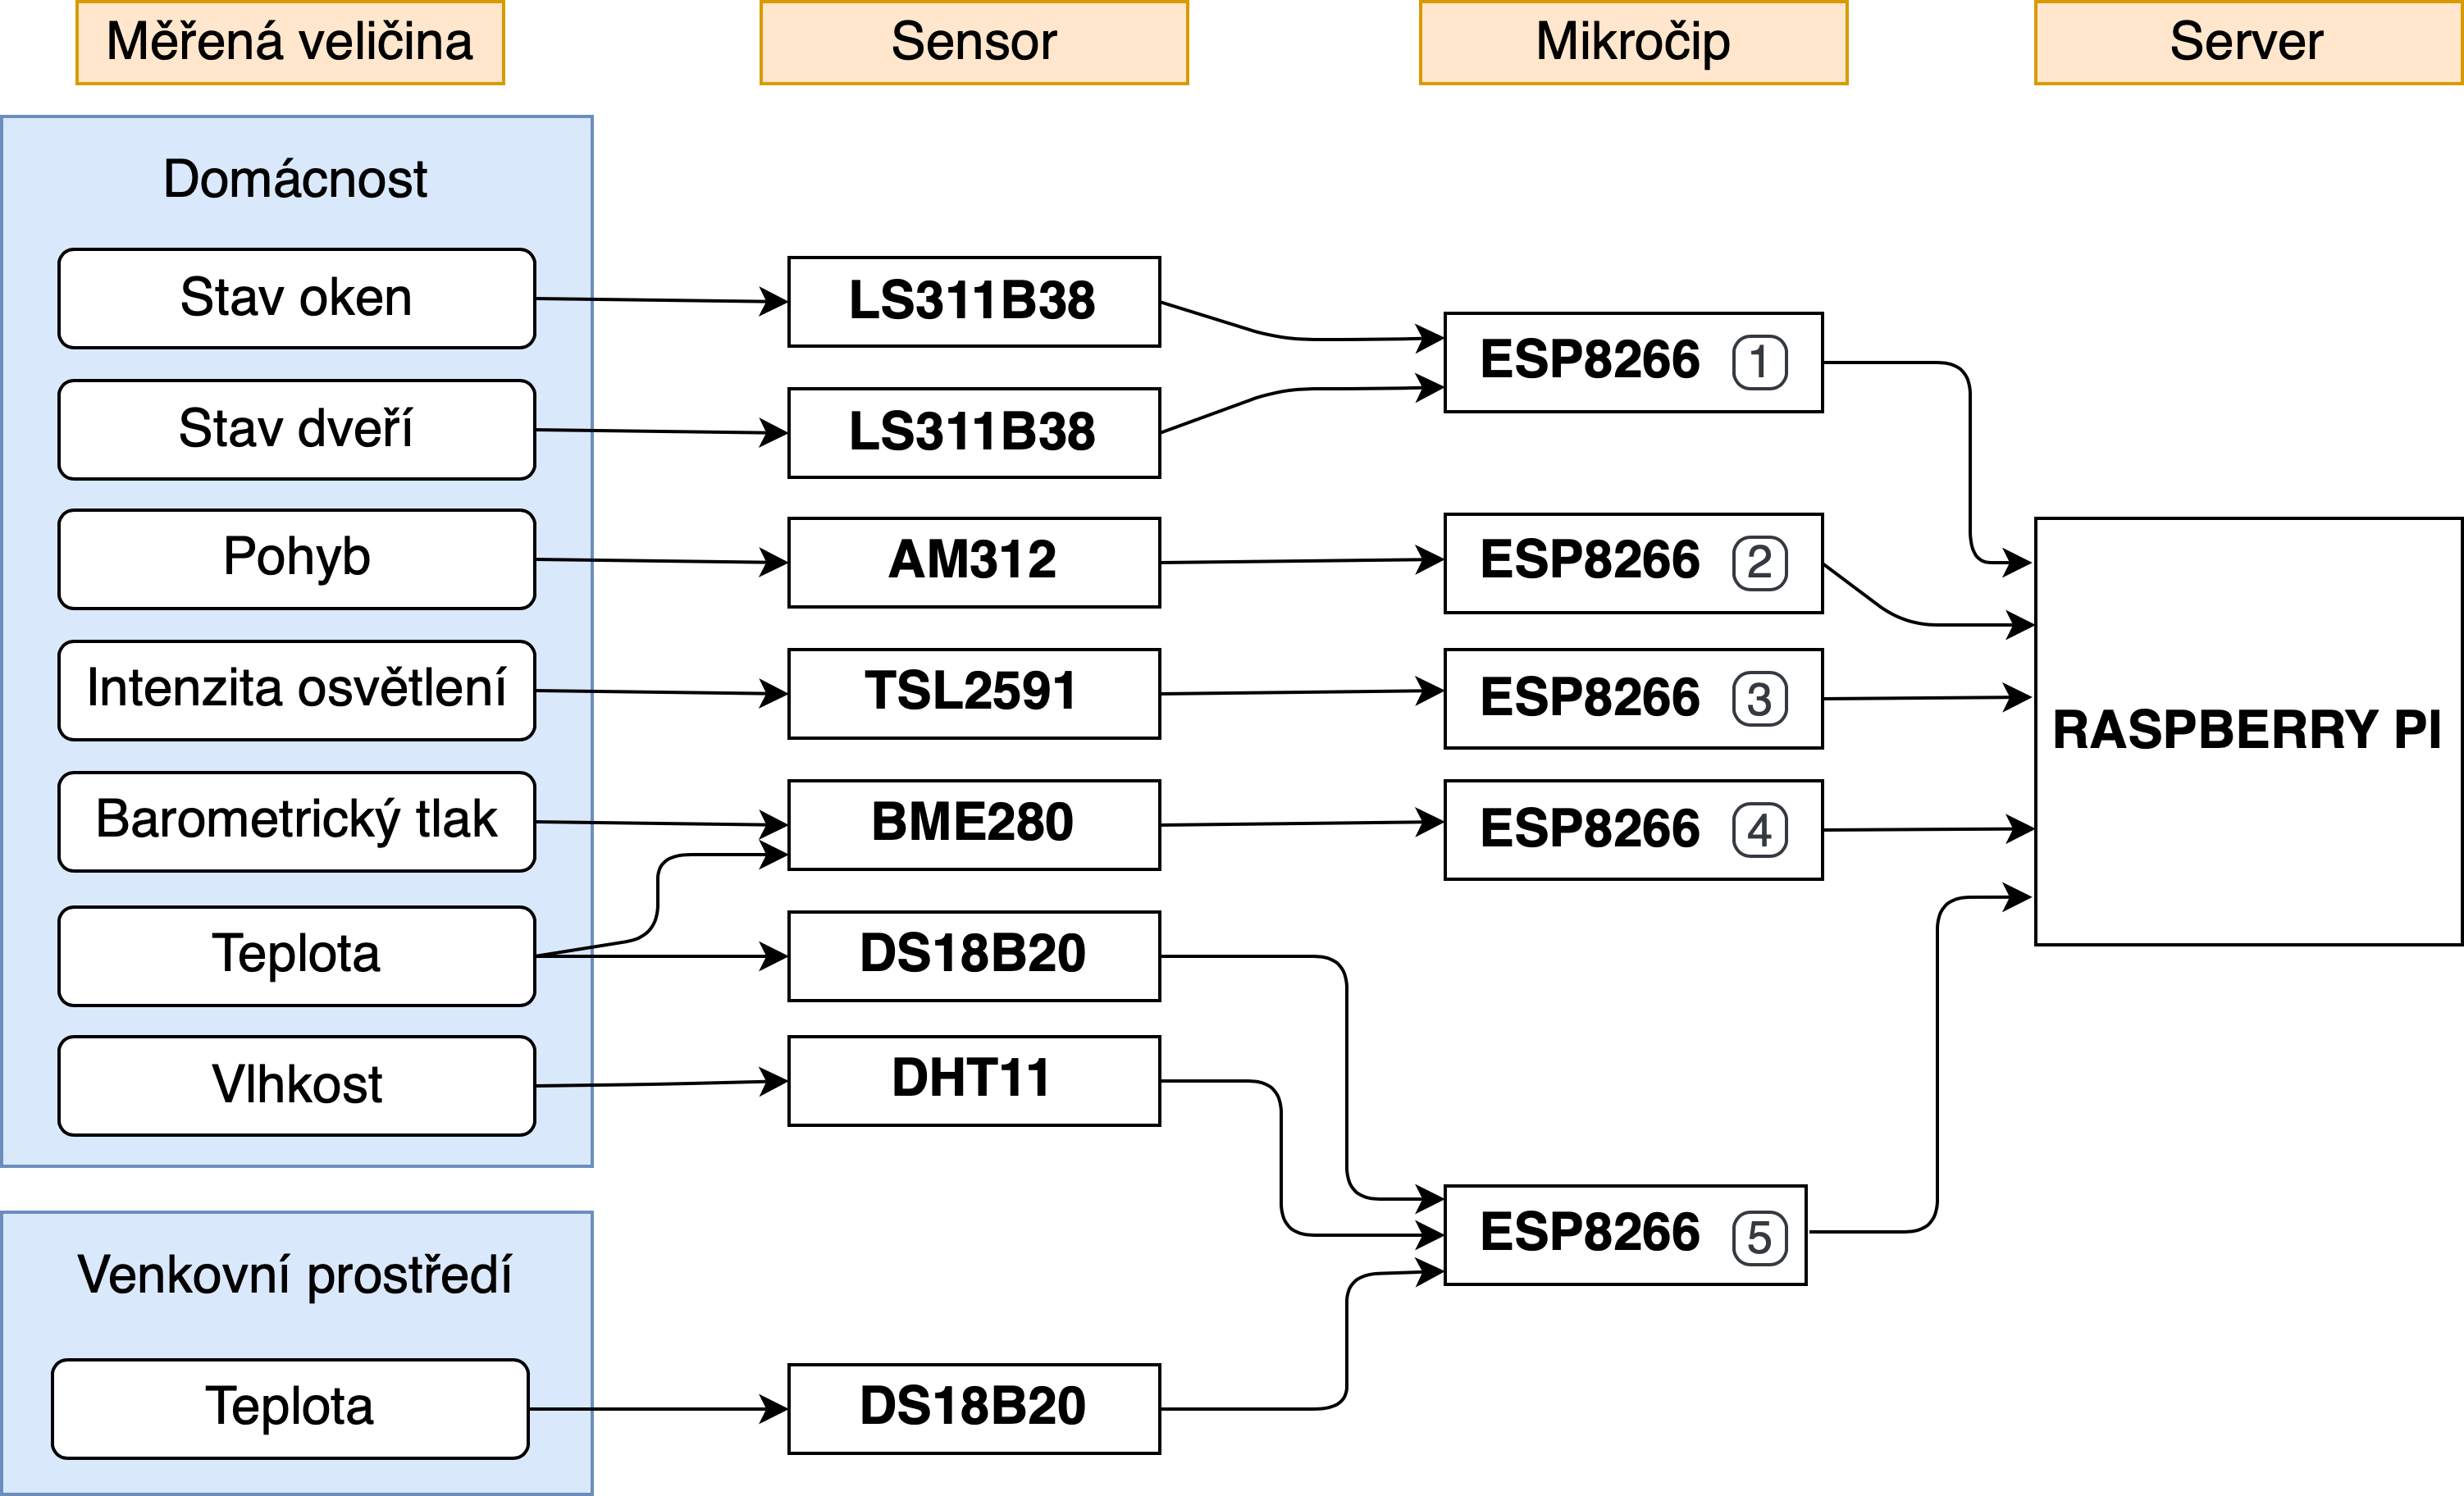
\includegraphics[width=0.9 \textwidth]{hardware_diagram.png}
  \caption{Vztahy mezi použitým hardwarem a měřenými veličinami}
  \label{fig:hardware_diagram}
\end{figure}

Ve snaze o co nejefektivnější využití hardwaru může jeden mikročip číst data z několika čidel. Tento přístup se využívá hlavně u čidel teploty a vlhkosti a u čidel pro monitorování stavu oken a dveří. U ostatních senzorů je zpravidla využitý jeden mikročip pro čtení dat z jednoho specifického čidla. Využitelnost jednoho mikročipu pro více čidel je závislá zejména na fyzickém umístění senzoru (např.: pohybový senzor musí být umístěn v rohu místnosti, kde není vhodné současně měřit jiné veličiny) a na výpočetní náročnosti. Jeden mikročip často zvládne načítat data pouze z jednoho čidla.

\section{Mikročip ESP8266} \label{sec:esp8266}

Základním stavebním prvkem senzorů v tomto projektu je mikročip \textit{ESP8266}. Existuje celá řada mírně odlišných mikrokontrolérů založených na tomto modulu, v principu se ale jedná o velmi levný mikročip s procesorem o frekvenci 80 Hz, flash pamětí typicky od 512 KiB do 4 MiB, 16 vstupně-výstupními piny a podporou sběrnic SPI,  I$^2$C a I$^2$S.

\subsection*{Vlastnosti mikročipu}
Hlavní předností tohoto čipu je podpora Wi-Fi standardu IEEE 802.11 b/g/n. K mikročipu stačí kabelově přivést pouze napájení a veškerá komunikace může probíhat bezdrátově po místní síti. Tím odpadá nutnost předem připravené kabeláže v domě a rozšiřují se možnosti využití i v méně dostupných prostorech. Tento druh mikročipu byl zvolen hlavně kvůli kompatibilitě s celou řadou čidel, podpoře několika programovacích jazyků a v neposlední řadě kvůli široce rozšířené komunitě a dostupnosti nejrůznějších návodů pro DIY projekty.

\subsection*{Vývojové platformy}
Vývojové desky s mikročipem ESP8266 jsou vyráběny v několika provedeních. V projektu senzorického řešení chytré domácnosti jsem využil výhradně vývojovou platformu \textit{NodeMCU} (na \cref{fig:nodemcu}). Tato platforma je přizpůsobena pro pohodlnou komunikaci s mikročipem ESP8266 pomocí sériové linky. Platforma disponuje USB konektorem a vývody GPIO pinů. USB konektor slouží k napájení a zároveň k přenosu dat do paměti mikročipu. Pro zapojení externích komponent a vytváření obvodů lze pohodlně využít breadboard\footnote{Nepájivé kontaktní pole. Komponenta, která umožňuje sestavit prototyp obvodu a je vhodná pro prvotní experimentování.} a propojovací kabely. Ve fázi vytváření prototypu tedy není nutné pájet.

\begin{figure}[H]
  \centering
  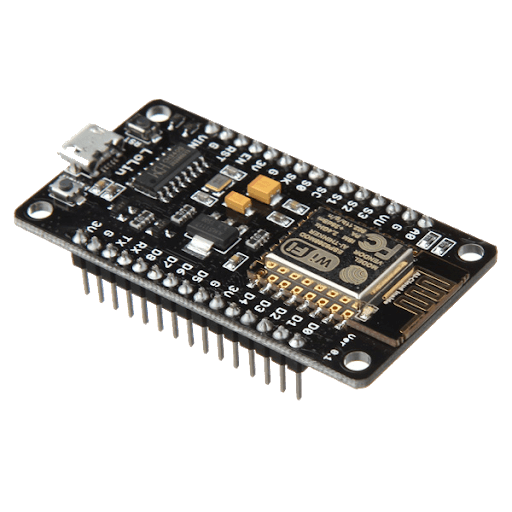
\includegraphics[width=0.4 \textwidth]{nodemcu.png}
  \caption{Vývojová platforma NodeMCU s modulem ESP8266}
  \label{fig:nodemcu}
\end{figure}

\subsection*{Firmware mikročipu}
Po zakoupení vývojové platformy je prvně potřeba nahrát aktuální firmware do flash paměti mikročipu. Před nahráním firmwaru je nutné nainstalovat ovladač pro komunikaci s USB rozhraním na desce. NodeMCU zpravidla vyžaduje ovladač CP2102 (alternativně CH340). Pro nahrání samotného firmwaru do mikročipu jsem zvolil nástroj \textit{esptool.py}. Esptool je program postavený na Pythonu, který umí načíst informace o připojeném mikročipu, vymazat flash paměť, nahrát nový firmware a případně zálohovat flash paměť.

\subsection*{Vývojové prostředí}
Veškerá komunikace s čipem probíhá po USB rozhraní a je založena na principu nahrání skriptů do paměti čipu a následném restartování pro spuštění programu. Jakákoliv změna kódu znamená vymazání původního skriptu z paměti čipu a následném nahrání nového skriptu. Tato skutečnost mírně ztěžuje ladění kódu a odchytávání chyb, ale samotný skript pro mikrokontrolér nebývá příliš dlouhý a k ladění kódu lze efektivně využít příkazovou řádku. Pro ukládání skriptů do mikročipu je potřeba vhodný nástroj pro přístup do adresářové části paměti na čipu. Jedním z těchto nástrojů je \textit{Mpfshell}. Mpfshell je balíček postavený na Pythonu, který umožňuje editaci souborů uložených v paměti (nahrávání, mazání, vytváření složek apod.) a zpřístupňuje příkazovou řádku na mikročipu. Právě příkazová řádka je zásadní pro rychlé spuštění kódu a odladění chyb, je možné v ní přímo psát části kódu nebo spouštět jednotlivé skripty bez nutnosti restartu.

\subsection*{Programování mikročipu} \label{subsec:microchip_programming}
Samotné ESP8266 může být programováno v několika jazycích, předně v Arduino IDE, MicroPythonu nebo LUA. V tomto projektu jsou všechny mikrokontroléry programovány v jazyce MicroPython. V rámci sjednocení programovacích jazyků v celém projektu jsem vybral MicroPython právě z důvodu univerzálnosti. MicroPython vychází z Pythonu 3 a je přímo přizpůsoben pro programování mikrokontrolérů. Další části projektu (například backend webové vizualizace nebo klasifikátor dat) jsou postaveny na Pythonu 3, proto se MicroPython v rámci zachování jednotné struktury jevil jako logická volba. Nespornou výhodou tohoto jazyku je velká podpora v rámci komunity a množství návodů a knihoven pro komunikaci s jednotlivými čidly. 

\subsection*{Odesílání dat z mikročipu}
V senzorech pro chytrou domácnost se uplatňují 2 základní přístupy odesílání dat na server. První je založen na odeslání zprávy na základě vzniku události a druhý přístup odesílá zprávy pravidelně s předem zvolenou periodou odesílání. V obou případech se po zapnutí senzoru mikročip nejprve připojí k Wi-Fi a problikne led dioadami. Tento proces proběhne jednorázově a pak senzor přejde do stavu, kdy je připraven načítat data ze senzorů a publikovat zprávy.

\subsubsection*{Odesílání zpráv na základě vzniku události} \label{subsec:event_based_msg}
Odesílání zpráv ze senzoru na server na základě vzniku události používá senzor pro detekci pohybu v místnosti a senzor pro monitorování stavu oken a dveří. Tento přístup je popsán v diagramu na \cref{fig:esp_event_based_diagram}. V nekonečném cyklu, do kterého se senzor dostane po připojení k internetu, se prvně sesynchronizuje čas se světovým časem pomocí protokolu NTP\footnote{\textbf{N}etwork \textbf{T}ime \textbf{P}rotocol - protokol pro synchronizaci času počítače po internetu}. Po synchronizaci senzor čeká, dokud se neobjeví událost, kterou má zaznamenat. Touto událostí je například otevření či zavření okna nebo dveří a nebo pohyb člověka v místnosti. V momentě, kdy událost nastane, čidlo problikne externí led diodou (v případě pohybového čidla se pro indikaci zapne ještě externí bzučák) a přejde do fáze vytváření zprávy. Po vytvoření struktury zprávy, která sestává z několika atributů (více v \cref{sec:protocol_mqtt}), se senzor připojí k MQTT brokeru a odešle zprávu. Po odeslání zprávy se uspí na 3 vteřiny a celý cyklus se opakuje. Uspání je v programu spíše jako preventivní opatření, aby se kód nežádaným způsobem nezacyklil. V případě pohybového senzoru je krátké uspání vhodné také pro to, aby čidlo neposílalo zbytečně moc zpráv, když v místnosti detekuje pohyb. Šetří se tím vytíženost sítě a pro účel detekce pohybuje není nutné odesílat informaci několikrát za vteřinu.

\begin{figure}[H]
  \centering
  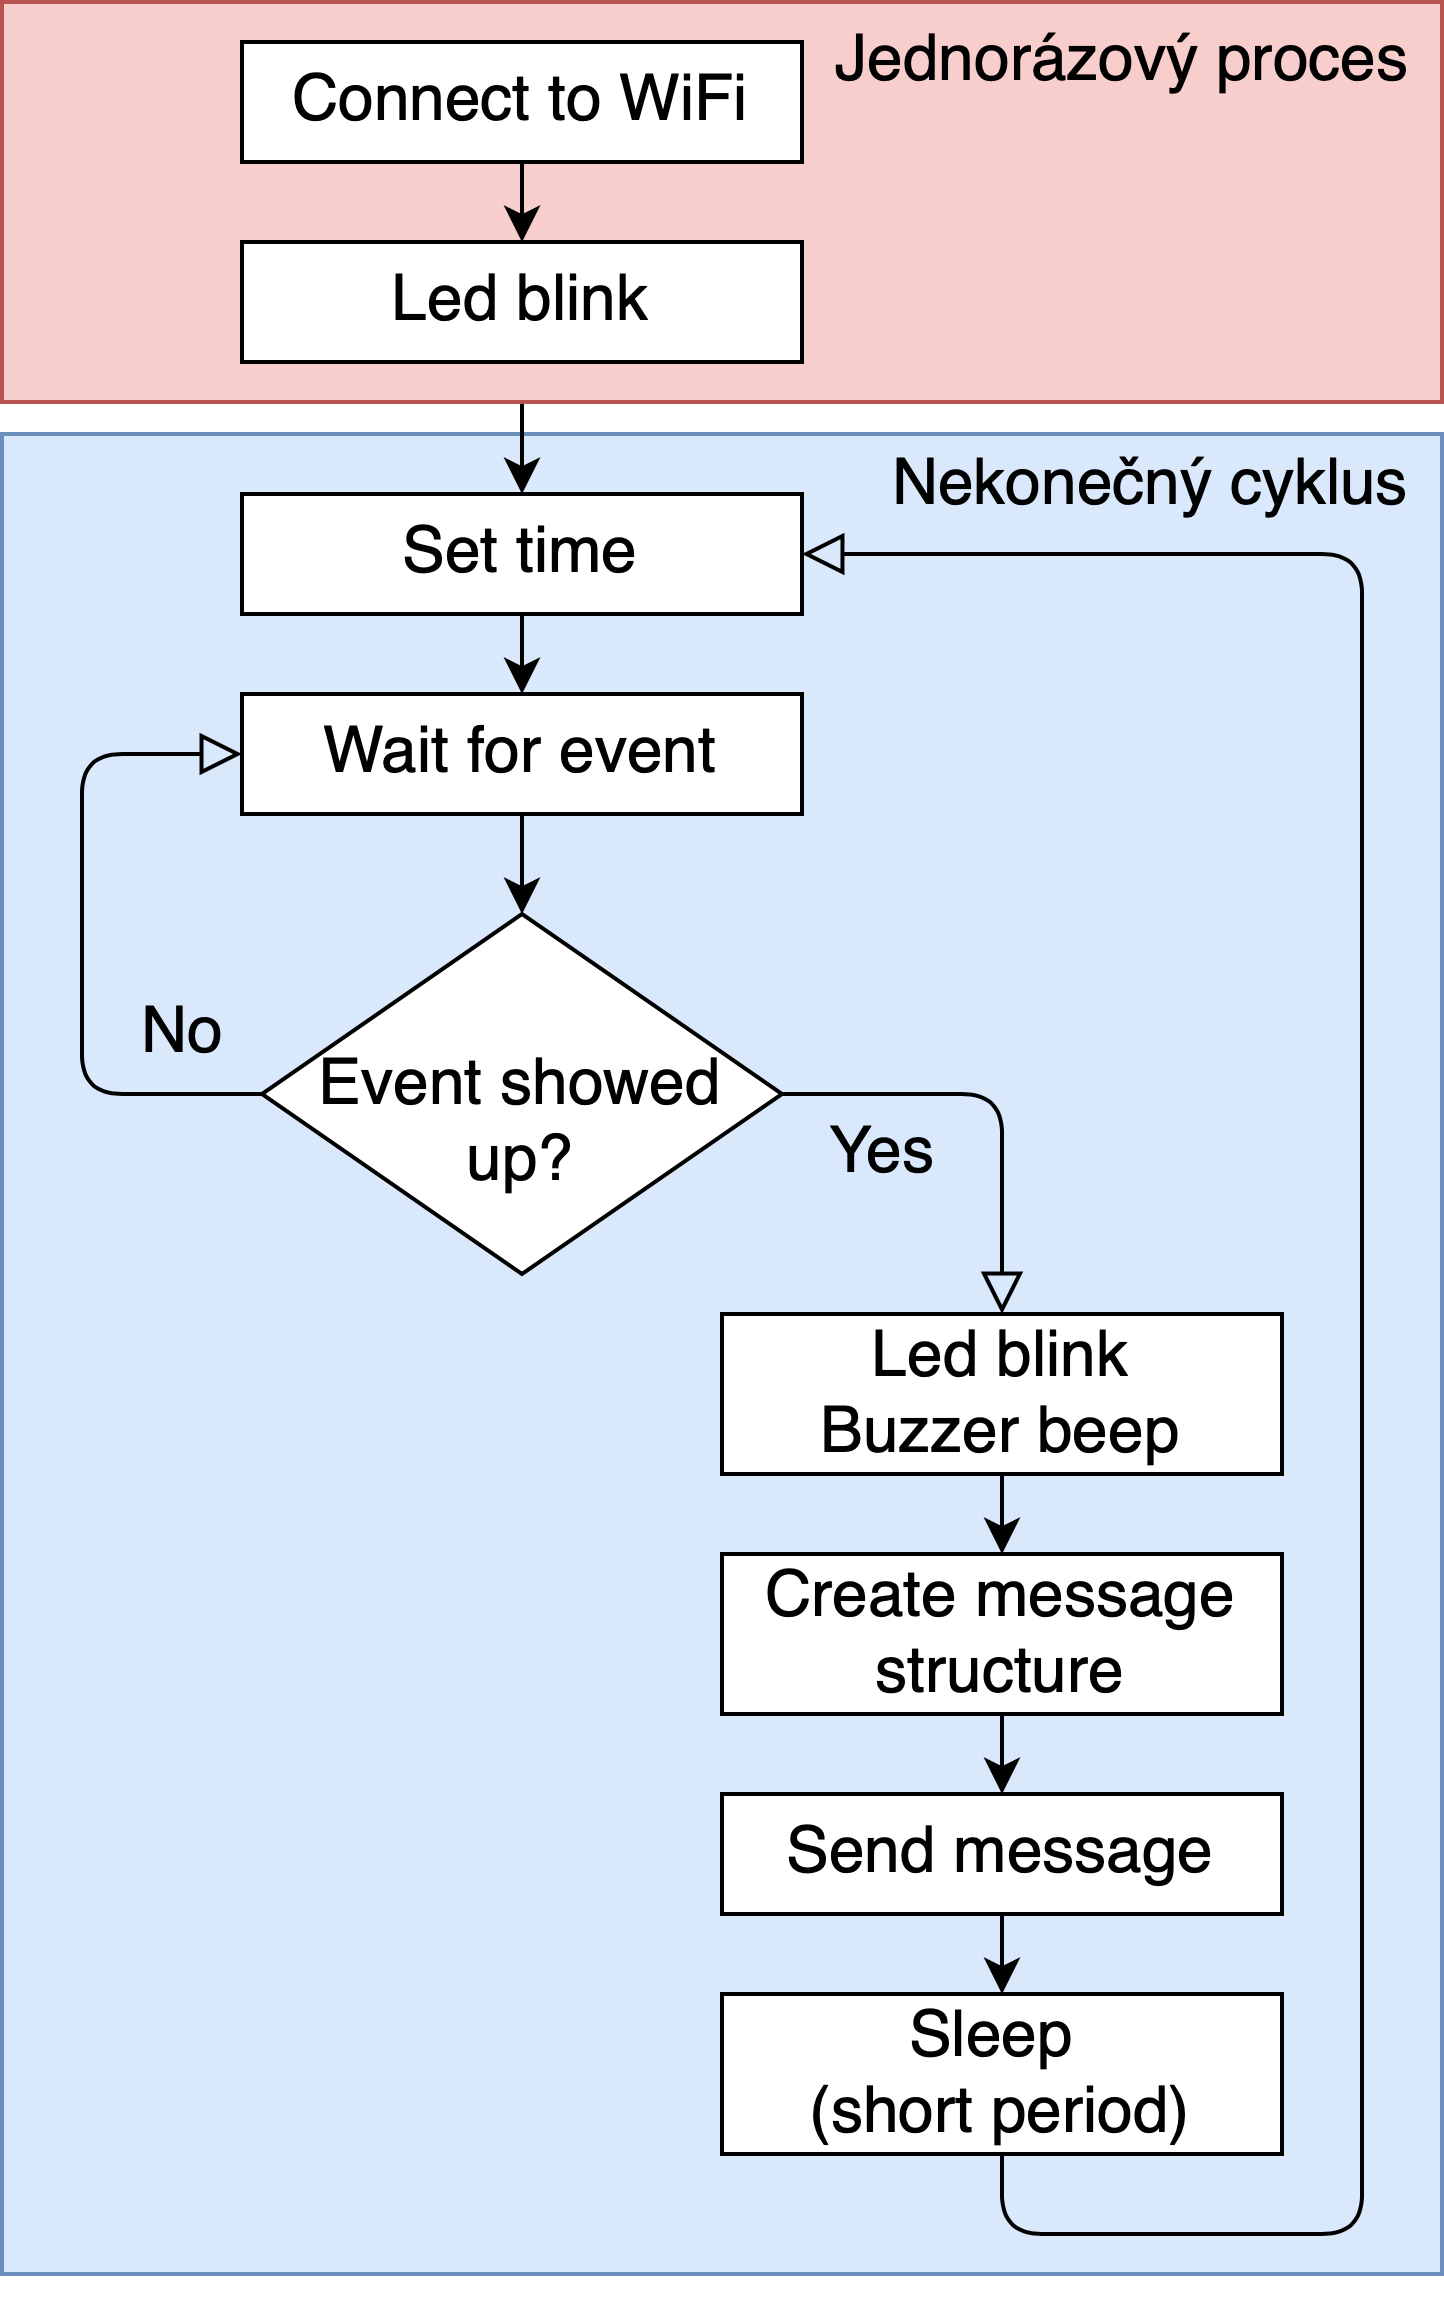
\includegraphics[width=0.5 \textwidth]{esp_event_based_diagram.png}
  \caption{Diagram odesílání zpráv na základě vzniku události}
  \label{fig:esp_event_based_diagram}
\end{figure} 
 
 \subsubsection*{Periodické odesílání zpráv} \label{subsec:periodical_based_msg}
Pravidelné odesílání zpráv s předem danou frekvencí odesílání používají všechny ostatní senzory měřící veličiny, u kterých je vhodné měření po určité době opakovat. Jde o čidla vnitřní a venkovní teploty, vlhkosti, intenzity osvětlení a barometrického tlaku. U těchto senzorů je vhodné měření fyzikálních veličin opakovat za účelem získání dostatečného množství dat pro následné trénování modelů a pro zajištění neustálé aktuálnosti hodnot ve webové vizualizaci. Vstupními parametry toho přístupu je perioda odesílání dat a určení okamžiku, ve kterém má proběhnout odeslání dat. V případě senzorů pro chytrou domácnost je perioda odesílání 1 minuta a okamžik, kdy se posílají data je vždy ve 30. vteřině (např.: po sobě jdoucí sekvence dat odeslaná v časech 14:25:30, 14:26:30, 14:27:30, ...). Minutová perioda odesílání dat je kompromis mezi dostatečným množstvím dat a vytížeností výpočetní techniky (vytíženost přenosové sítě, množství potřebné kapacity pro ukládání těchto dat, opotřebení čidel vlivem neustálého načítání dat apod.). Odesílání dat každou minutu vytvoří 1440 vzorků dat za 24 hodin. Po několika dnech sbírání dat už lze z tohoto množství dat počítat statistiky a trénovat klasifikátory. Specifická volba odesílání dat ve 30. vteřině je spíše návrhové rozhodnutí, které sjednocuje odesílání dat ze všech senzorů ve stejném okamžiku. Přístup periodického odesílání dat je popsán v diagramu na \cref{fig:esp_periodical_diagram}.

\begin{figure}[H]
  \centering
  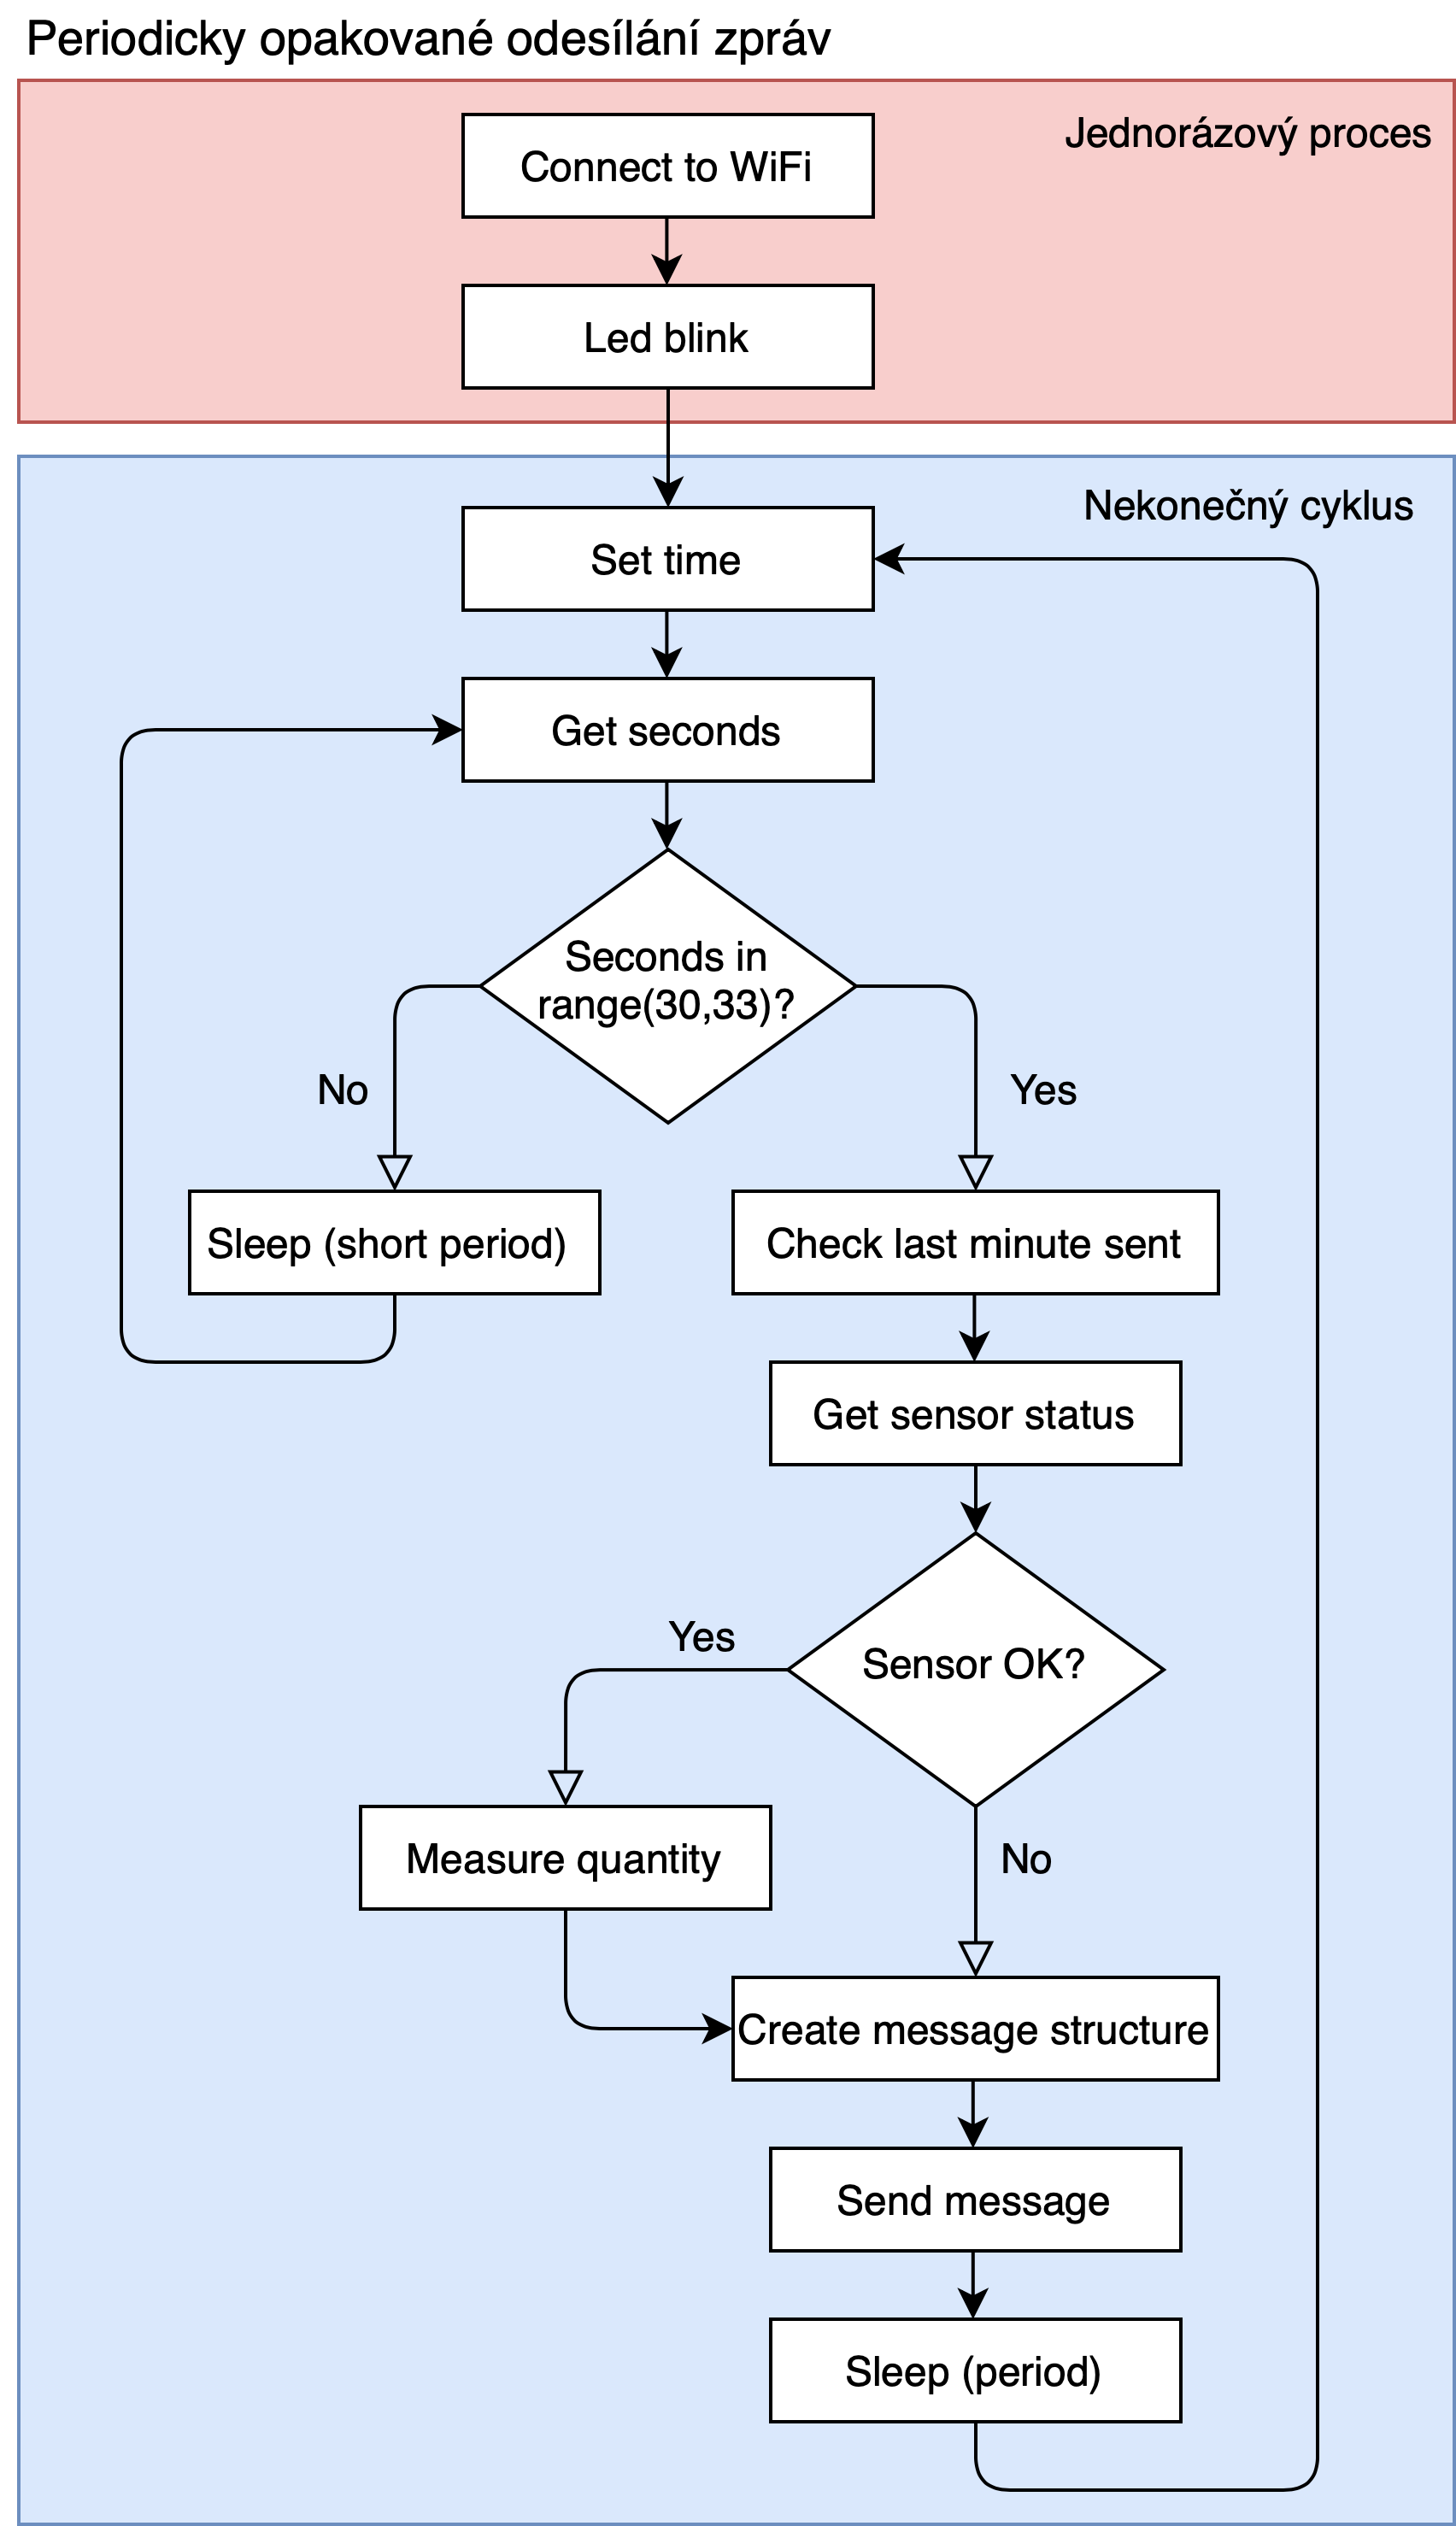
\includegraphics[width=0.5 \textwidth]{esp_periodical_diagram.png}
  \caption{Diagram periodicky opakovaného odesílání zpráv}
  \label{fig:esp_periodical_diagram}
\end{figure}

V nekonečném cyklu, do kterého se senzor dostane po připojení k Wi-Fi, se nejdříve sesynchronizují vnitřní hodiny mikročipu se světovým časem pomocí protokolu NTP. Následně senzor čeká v cyklu na okamžik, kdy má odeslat zprávu (30. vteřina každé minuty). V momentě, kdy je podmínka splněna a je čas na zprávu, mikročip zjistí status senzoru a načte data (zjištění statusu čidla je přímo spojeno s načtením dat - pokud se podaří načíst data z čidla, status čidla je "OK", pokud dojde k chybě při pokusu o načtení dat, status čidla je "ERROR". Více o detekci chyb na úrovni mikročipu v \cref{sec:error_detection_esp}). Po načtení dat z čidla se vytvoří struktura zprávy (více o struktuře zprávy v \cref{sec:protocol_mqtt}) a zpráva se odešle na MQTT broker. Po odeslání se senzor uspí na čas $t-10$[sec], kde $t$ je perioda odesílání. Například pro periodu odesílání 1 minuta se senzor uspí na 50 vteřin. Zbylých 10 vteřin, kdy senzor nespí, je určeno pro proces načtení dat ze senzoru (např.: u teplotního senzoru, který načítá data z několika čidel tento proces trvá v průměru 3 až 4 vteřiny), vytvoření zprávy a odeslání zprávy.

\subsection*{Architektura kódu na mikročipu}
Architektura kódu všech senzorů sestává ze stejného jádra. Při návrhu programu pro mikročipy byl kladen důraz na objektovou strukturu programování a co nejuniverzálnější využití. Proto je základ programu pro všechny senzory stejný a liší se jen komunikací s konkrétním čidlem. Tímto přístupem se podařilo sjednotit verze kódu ve všech senzorech a hlavně umožnit rychlé přidání dalších senzorů v budoucnu. Pokud bych do chytré domácnosti chtěl přidat další senzor, který bude měřit jinou fyzikální veličinu, nemusím programovat celou logiku senzoru znovu nebo složitě vytrhávat části jinde použitého kódu, ale použiji stávající program, který pouze doplním o implementaci komunikace s konkrétním čidlem. Vizuální pohled na architekturu kódu na mikročipu je na \cref{fig:esp_code_architecture}. 

\begin{figure}[H]
  \centering
  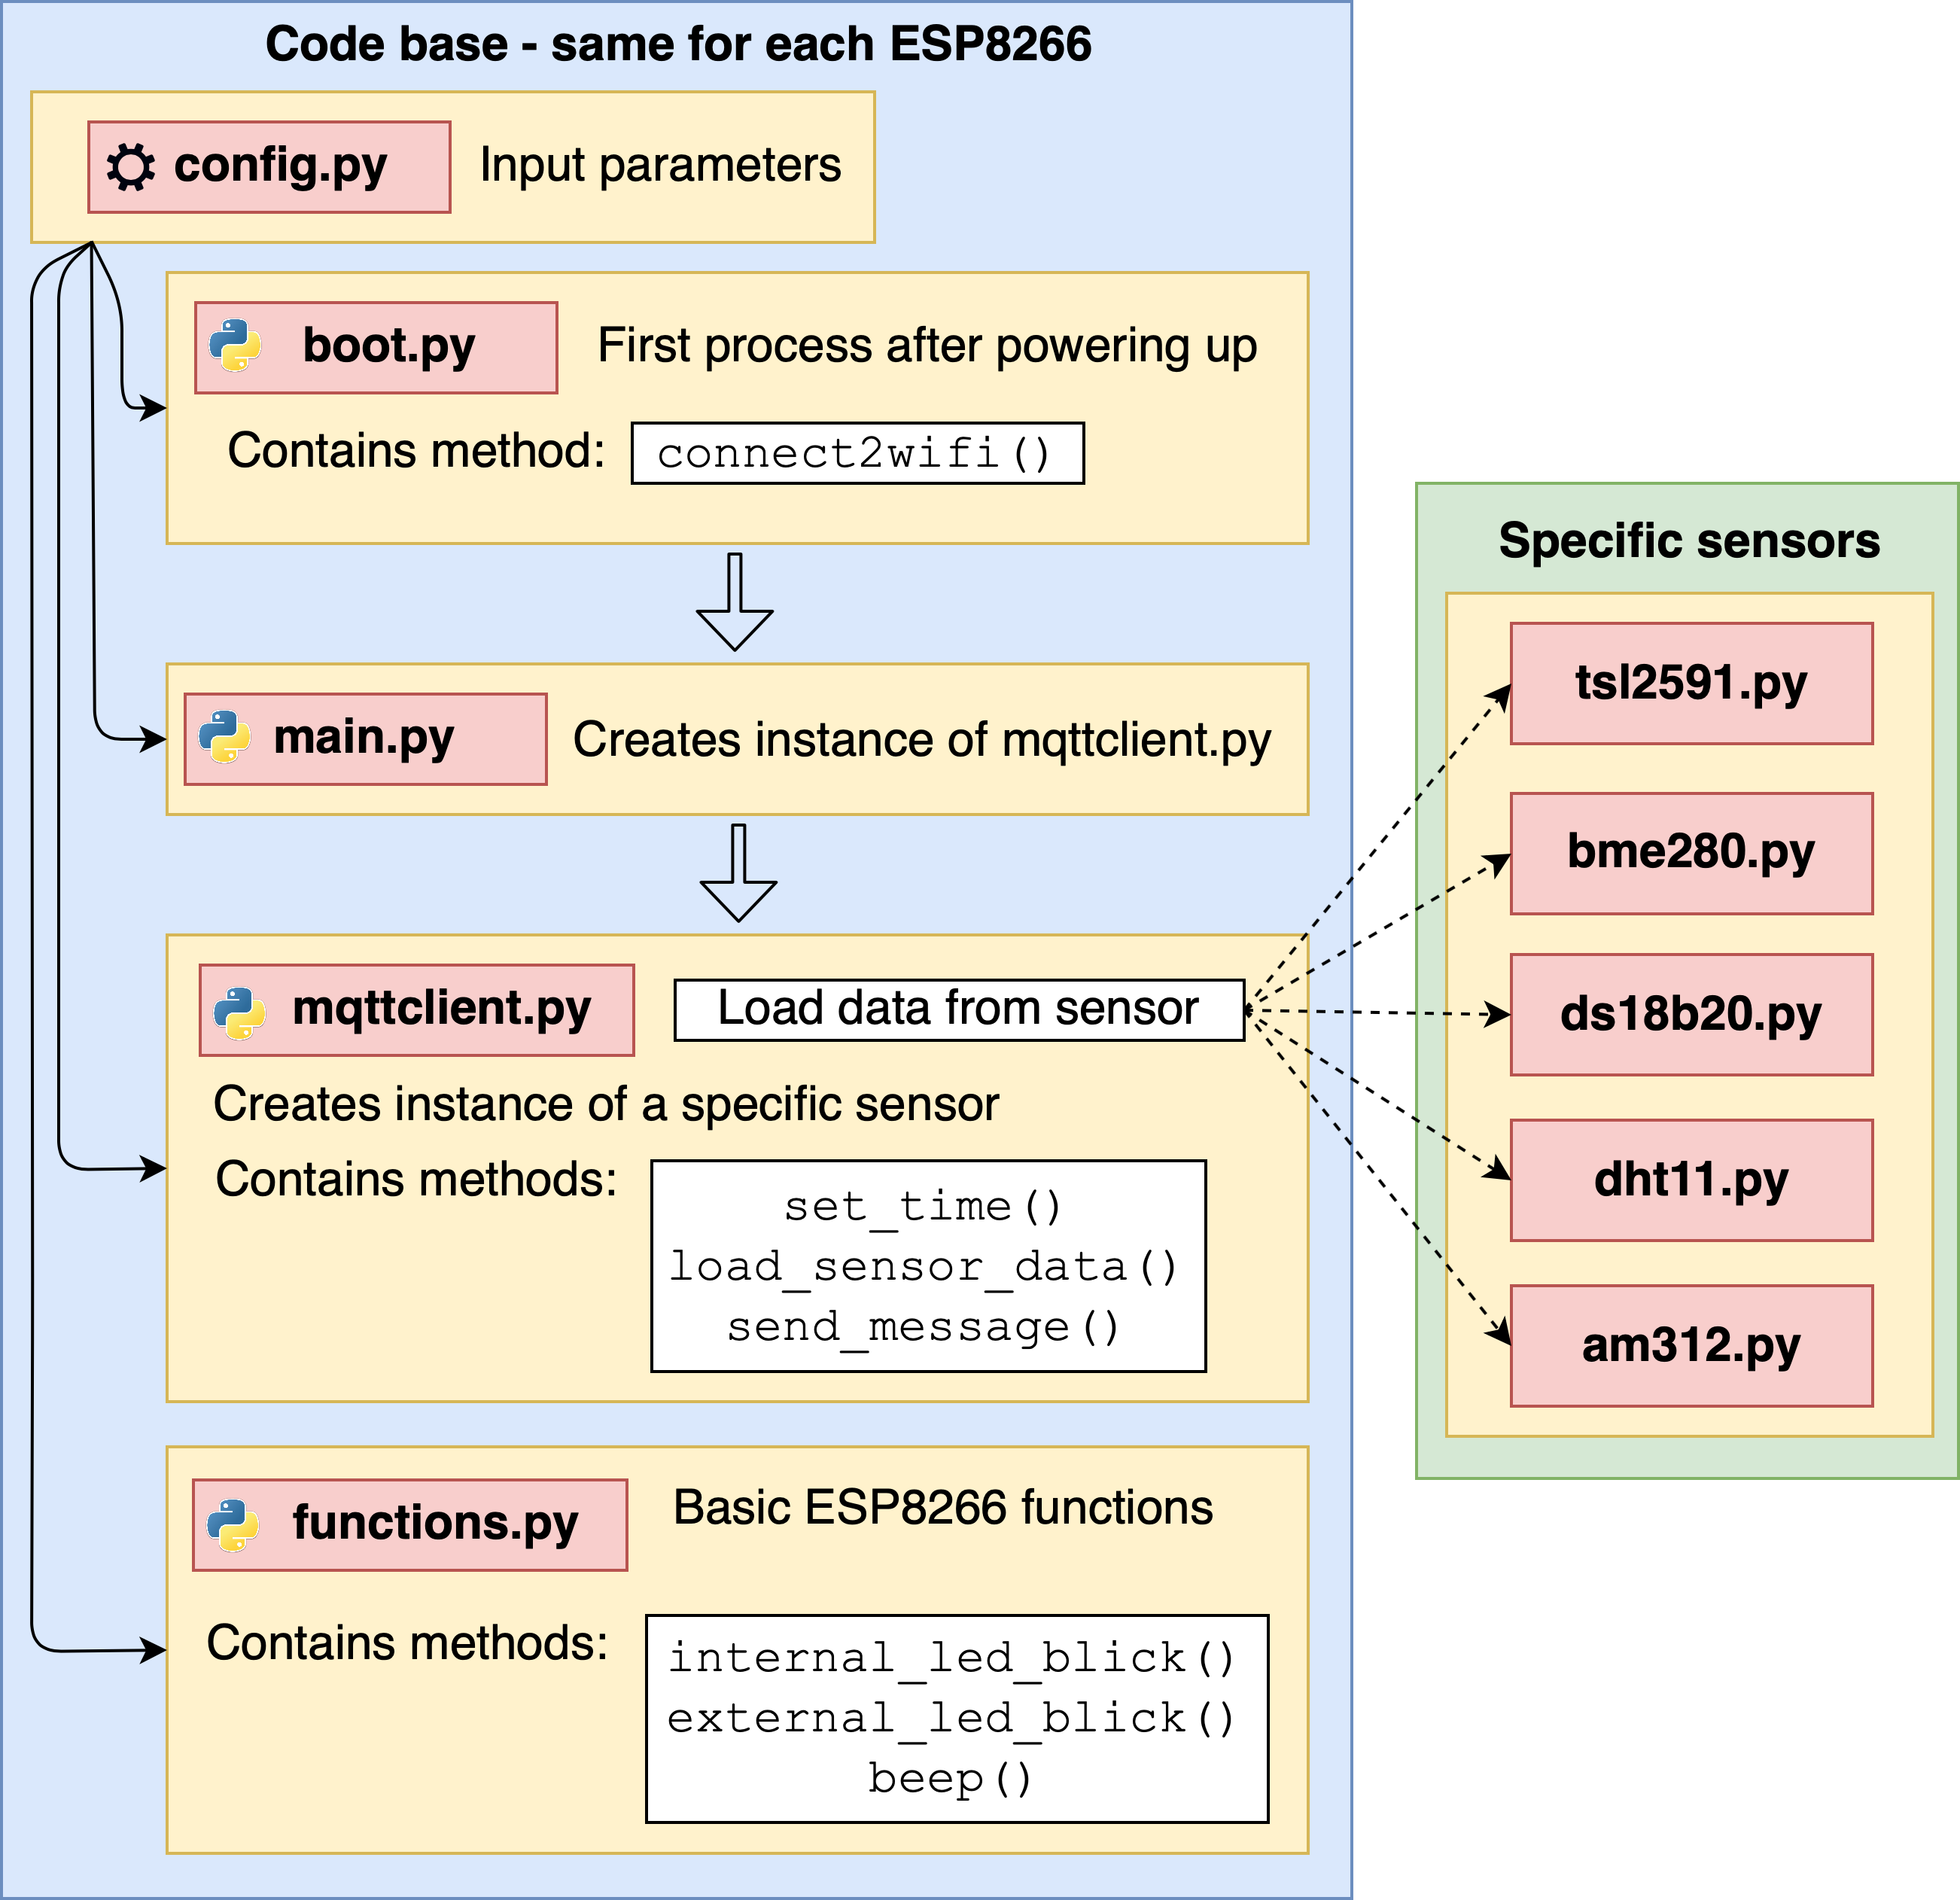
\includegraphics[width=0.9 \textwidth]{esp_code_architecture.png}
  \caption{Diagram architektury kódu na microchipu ESP8266}
  \label{fig:esp_code_architecture}
\end{figure}

Struktura kódu pro mikročip ESP8266 se skládá z 6 souborů - \textit{boot.py}, \textit{main.py}, \textit{mqttclient.py}, \textit{functions.py}, jednoho skriptu pro komunikaci s čidlem a jednoho konfiguračního souboru. Skripty \textit{boot.py} a \textit{main.py} jsou pevně dané programovacím jazykem MicroPython. 
 
\begin{itemize}
  \item \textit{config.py} 
  
V souboru \textit{config.py} jsou nadefinovány vstupní parametry konkrétního senzoru. Jsou zde uloženy přístupové údaje pro připojení k Wi-Fi, parametry pro MQTT komunikaci a označení GPIO pinů podle reálného využití (mikročip a čidlo je napájené na plošném spoji a využití GPIO je pevně dané touto fyzickou realizací). Všechny parametry jsou uloženy v tomto konfiguračním souboru a zbytek kódu pouze odkazuje na tyto parametry.  
  
  \item \textit{boot.py}
  
Skript \textit{boot.py} se po zapnutí mikrokontroléru spustí vždy jako první nezávisle na jakémkoliv jiném souboru. V tomto skriptu dochází k připojení k místní Wi-Fi síti. Po úspěšném připojení k síti senzor čtyřikrát zabliká interní led a následně i externí led diodou pro vizuální kontrolu.  
  
  \item \textit{main.py}
 
Druhým skriptem, který naběhne ihned po \textit{boot.py} je \textit{main.py}. Toto pořadí spuštění skriptů je pevně stanovené programovacím jazykem. Ve skriptu \textit{main.py} se vytvoří instance třídy MQTTClient. 
  
  \item \textit{mqttclient.py}
  
Tato třída je v podstatě jádrem celého programu pro mikročip. Dochází zde k synchronizaci vnitřních hodin se světovým časem, načítání dat z čidla, vytváření struktury zprávy a publikování zprávy. Ve třídě MQTTClient se vytvoří instance třídy konkrétního čidla, která obstarává veškerou komunikaci s čidlem. Třída MQTTClient je tedy pro všechny mikročipy stejná, jednotlivé mikročipy se liší jen třídou pro komunikaci s konkrétním čidlem.   
  
  \item \textit{functions.py}
  
Soubor \textit{functions.py} obsahuje obecné funkce mikročipu ESP8266. Umožňuje zapnutí interní a externí led diody a zapnutí externího bzučáku. Funkce jsou napsané univerzálně a načítají vstupní parametry ze souboru \textit{config.py}. Z konfiguračního souboru se načítá například číslo GPIO pinu externí led diody - každý senzor může mít externí led diodu umístěnou na jiném GPIO pinu, kvůli využití místa na plošném spoji, ale metoda pro rozsvícení diody je vždy stejná.  
\end{itemize} 
 
Soubory \textit{tsl2591.py}, \textit{bme280.py}, \textit{ds18b20.py}, \textit{dht11.py} a \textit{am312.py} jsou skripty pro komunikaci s konkrétním čidly a mikročip obsahuje vždy jen ten komunikační skript, který pro obsluhu svého čidla potřebuje. \par
Využitím objektově orientovaného programování a implementací konfiguračních souborů bylo dosaženo maximální univerzálnosti a přehlednosti kódu skrze všechny senzory v chytré domácnosti. Hlavní výhodou tohoto přístupu je snadná rozšiřitelnost kódu v budoucnu a díky udržení jedné vývojové větve je na každém mikročipu možné snadno aktualizovat kód. Díky konfiguračnímu souboru je možné měnit vstupní parametry bez nutnosti zásahu do samotného kódu. 

\section{Senzory} \label{sec:sensors}
V projektu chytré domácnosti bylo použito celkem 7 typů čidel pro měření fyzikálních veličin. Mezi tyto čidla patří teplotní čidlo \textit{DS18B20}, vlhkoměr \textit{DHT11}, čidlo intenzity osvětlení \textit{TSL2591}, čidlo barometrického tlaku a teploty \textit{BME280}, pohybové čidlo \textit{AM312} a magnetické čidlo pro monitorování stavu oken a dveří \textit{LS311B38}. Tyto fyzikální veličiny mají z pohledu chytré domácnosti význam pro automatizaci, zajištění bezpečnosti objektu a přehled o podmínkách uvnitř domu a okolí. Data z těchto senzorů jsou následně využita pro trénovaní modelů, klasifikaci jednotlivých hodnot a pro predikci měřených hodnot. Konkrétní senzory byly vybrány na základě kompromisu mezi cenou, funkčností a přesností měření. 

\subsection*{Postup fyzické realizace čidel}
Prvním krokem při návrhu chytrých čidel je stanovení fyzikálních veličin, které chceme sledovat a otestovat spolehlivost čidel pro měření těchto veličin. Po vybrání konkrétních senzorů následuje sestrojení prototypu - zapojení obvodu na breadboardu. Po vytvoření funkčního obvodu může začít experimentování a ladění kódu pro načítání dat z čidla. Po úspěšném naprogramování komunikace s čidlem jsem přešel k vytvoření pevného fyzického obvodu napájením jednotlivých součástí na plošný spoj. Tento plošný spoj má nespornou výhodu ve své životnosti a odolnosti, na rozdíl od obvodu na breadboardu, kde se kabely mohou vlivem neopatrnosti vypojovat. Ke každému senzoru jsem přidal červenou externí led diodu pro indikaci různých změn a stavů. Uživatel v podstatě nemá žádný jiný způsob vizuální kontroly funkčnosti senzoru. Led diodu využívám jako signalizaci při úspěšném připojení k Wi-Fi a jako signalizaci odeslání zprávy. Vždy, když senzor odešle zprávu, dioda jednou blikne.

\subsection{Teplotní čidlo DS18B20}
Teplotní čidlo Dallas DS18B20 se vyrábí ve více provedení, v projektu chytré domácnosti jsou použity 2 čidla, jedno v klasickém provedení pro měření vnitřní teploty a jedno voděodolné pro měření venkovní teploty. Rozsah měření tohoto čidla je od -55 \si{\degree}C do +125 \si{\degree}C s přesností $\pm$ 0,5 \si{\degree}C v mezích od -10 \si{\degree}C do +85 \si{\degree}C. Doba nutná pro konverzi 12 bitové hodnoty teploty do digitálního čísla je 750 ms. Datová komunikace probíhá přes rozhraní One-Wire a pro přenos dat je využitý jeden pin. Každé čidlo DS18B20 má svoji unikátní 64 bitovou sériovou adresu. Díky tomu je umožněno vytvořit One-Wire obvod s několika čidly, které jsou připojeny k jednomu digitálnímu GPIO pinu a pomocí toho sériového čísla lze čidlo snadno identifikovat při programování komunikace čidla s mikročipem. \par
Čidlo je k mikročipu připojeno třemi dráty - jeden drát pro napájení, jeden pro uzemnění a jeden pro datovou komunikaci. Napájecí drát je na ESP8266 připájen k pinu 3,3V, zemnící drát ke GND a datová linka je připájena k digitálnímu pinu D4. Do obvodu je potřeba připojit rezistor s odporem 4,7k \si{\ohm}, který spojuje datový a napájecí drát. Schéma zapojení obou čidel DS18B20 je zobrazeno na \cref{fig:schema_esp_ds18b20}.\par

\begin{figure}[H]
  \centering
  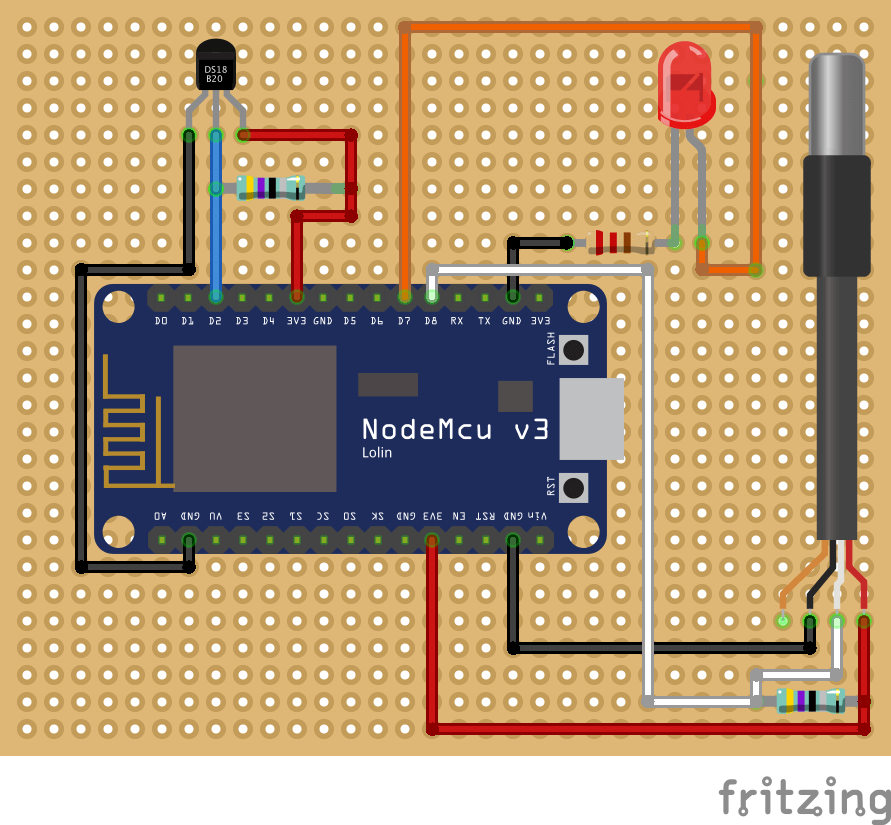
\includegraphics[width=0.6 \textwidth]{ds18b20.png}
  \caption{Schéma obvodu platformy NodeMCU, dvou čidel DS18B20 a led diody na plošném spoji}
  \label{fig:schema_esp_ds18b20}
\end{figure}

Čidlo DS18B20 se osvědčilo přesností měření a důvěryhodností naměřených hodnot. Při prvotním testování jsem zapojil najednou více těchto čidel blízko sebe a naměřené hodnoty ze všech čidel se lišily v rámci desetin stupně. V projektu chytré domácnosti jsou hodnoty teplot zaokrouhlovány na 2 desetinná místa, tudíž přesnost v rámci desetin dostačuje a odchylky jsou zanedbatelné. V tomto projektu jsou teplotní čidla DS18B20 a vlhkostní snímač DHT11 z důvodu efektivního využití hardwaru a stejnému umístění v místnosti připojeny k jednomu mikročipu ESP8266. Senzor skládající se z jedné platformy NodeMCU, jednoho vnitřního čidla DS18B20, jednoho venkovního čidla DS18B20, jednoho vlhkoměru DHT11 a externí led diody je umístěn v rohu místnosti. Venkovní čidlo má 1 m dlouhý kabel a je umístěno za oknem. Na \cref{fig:nodemcu_ds18b20_dht11} je vyfocena fyzická realizace zkonstruovaného senzoru.

\begin{figure}[H]
  \centering
  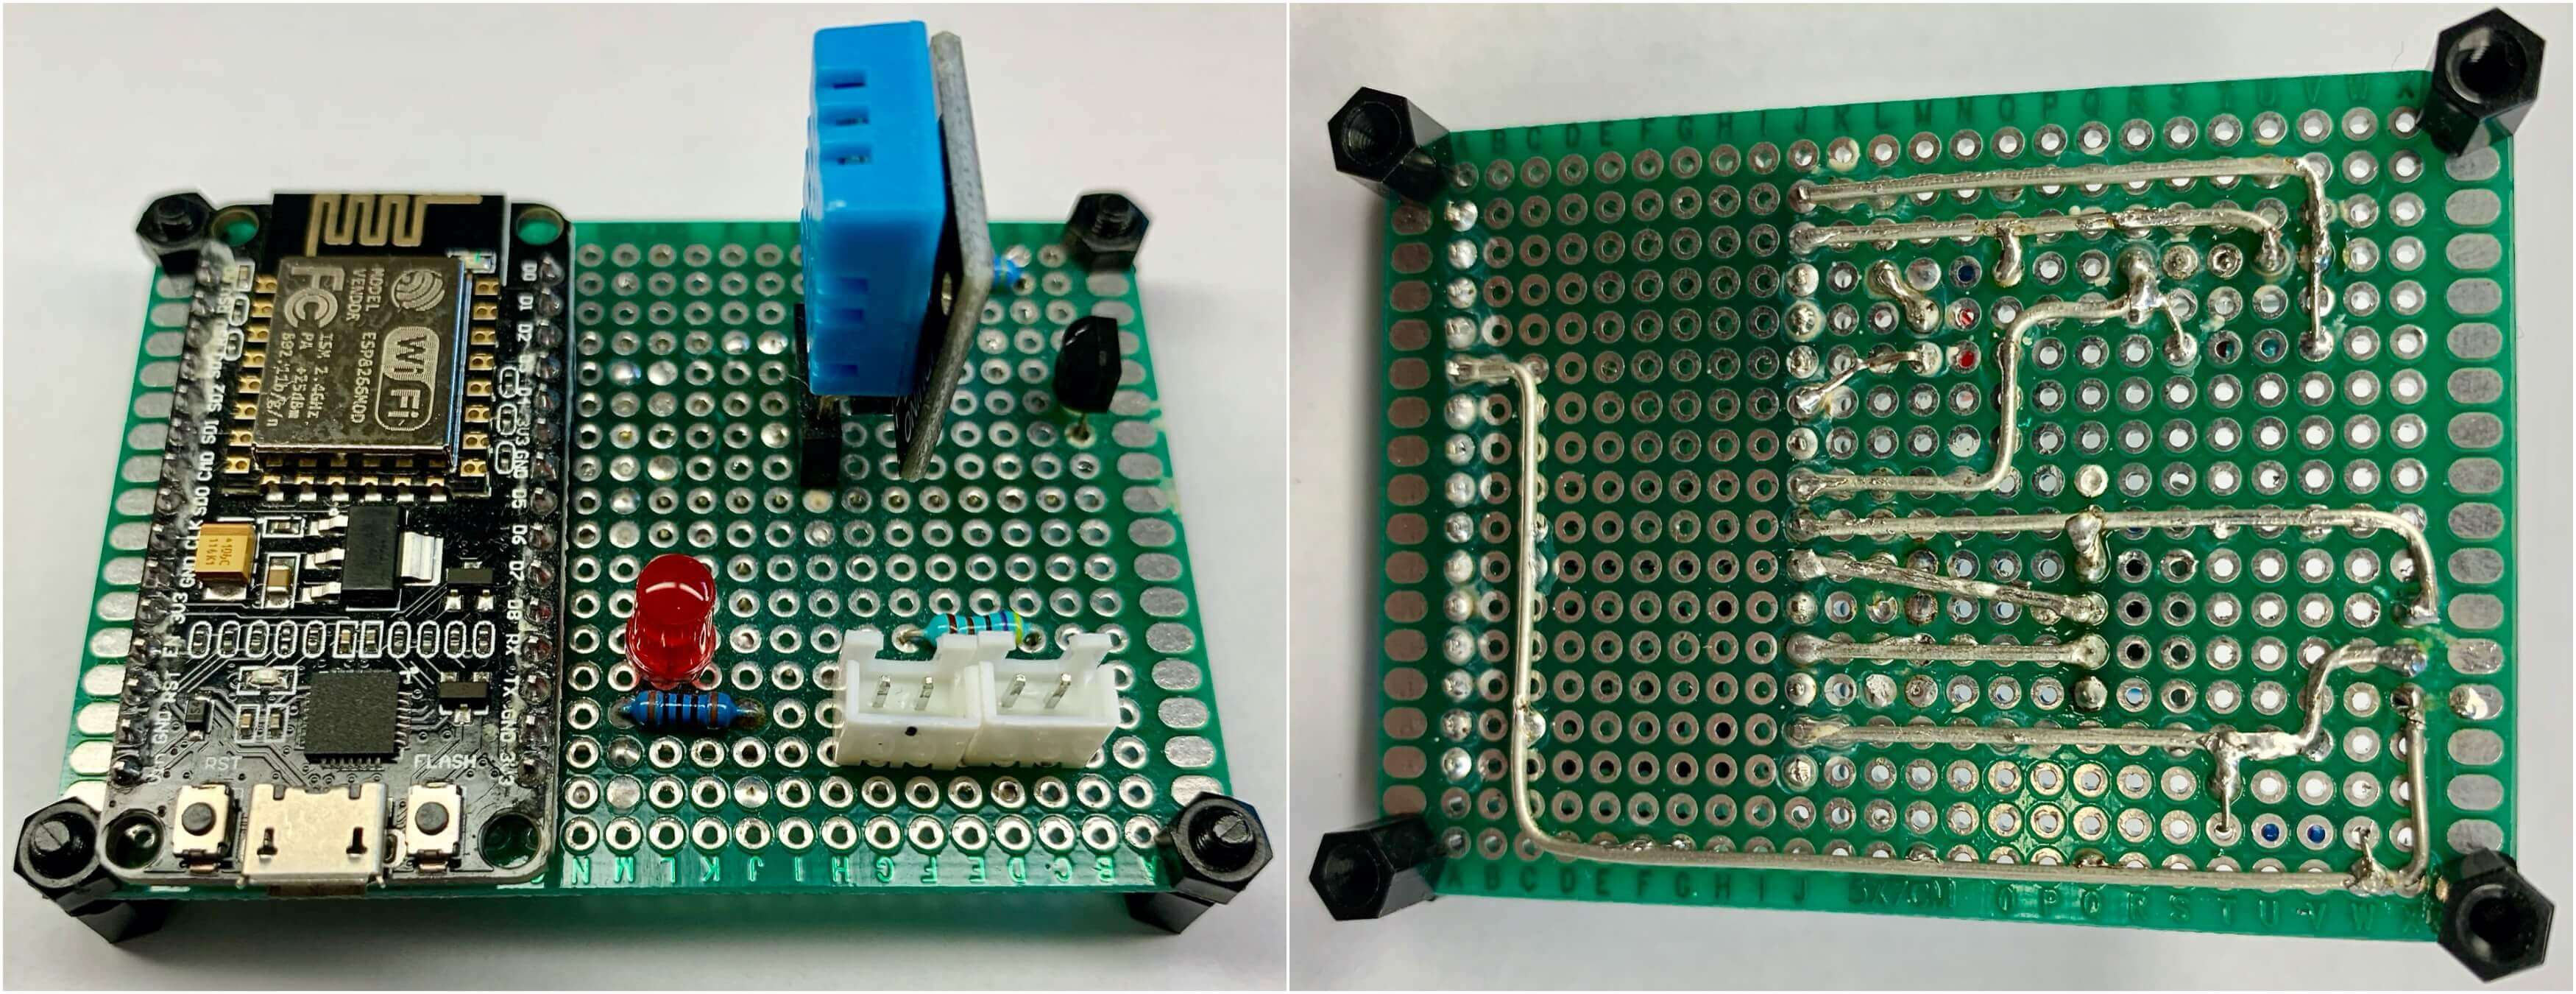
\includegraphics[width=0.9 \textwidth]{nodemcu_ds18b20_dht11.jpg}
  \caption{Fyzická realizace senzoru s moduly DS18B20 a DHT11}
  \label{fig:nodemcu_ds18b20_dht11}
\end{figure} 

\subsection{Vlhkoměr DHT11} \label{subsec:dht11}

Modul DHT11 je určen pro měření vlhkosti a teploty uvnitř místnosti. Měřit teplotu umožňuje v rozmezí od 0 \si{\degree}C do +50 \si{\degree}C s přesností $\pm$ 2,0 \si{\degree}C. Z důvodu menšího rozsahu měření a hlavně nižší přesnosti je toto čidlo v projektu chytré domácnosti používáno pouze pro měření vlhkosti. Vnitřní vlhkost je měřena v rozmezí 20 \% až 90 \% s přesností $\pm$ 5 \%. Chyba měření vlhkosti také není zcela zanedbatelná, nicméně pro základní představu o vlhkosti v místnosti postačuje. Často nezáleží na konkrétní hodnotě vlhkosti, ale spíše na změně této hodnoty v průběhu dne. Pokud je například celý den domácnost bez přítomnosti lidí, drží se vlhkost celý den na stejné hodnotě. Po příchodu člověka do místnosti se hodnota vlhkosti zvýší (sice mírně v rámci jednotek procent, ale s touto informací už je možné dále pracovat). \par
Čidlo DHT11 je k mikročipu připojeno třemi dráty - jeden drát pro napájení, jeden pro uzemnění a jeden pro přenos dat. Modul vyžaduje napětí v rozmezí 3,0 V až 5,5 V. Po zavedení napětí k modulu je před měřením vyžadováno minimálně 1 vteřinu počkat na kalibraci čidla. Tuto prodlevu je nutné brát v úvahu při každém načítání dat z čidla. Ze zkušenosti s komunikací s čidlem DHT11 raději používám 2 vteřinovou pauzu, při kratším intervalu se často stávalo, že čidlo nestihlo odpovědět a kód spadl do chyby. Metoda pro čtení hodnot z čidla DHT11 vrací hodnotu v procentech zaokrouhlenou na celá čísla. Schéma zapojení modulu DHT11 a vývojové platformy NodeMCU je zobrazeno na \cref{fig:schema_esp_dht11}. \par

\begin{figure}[H]
  \centering
  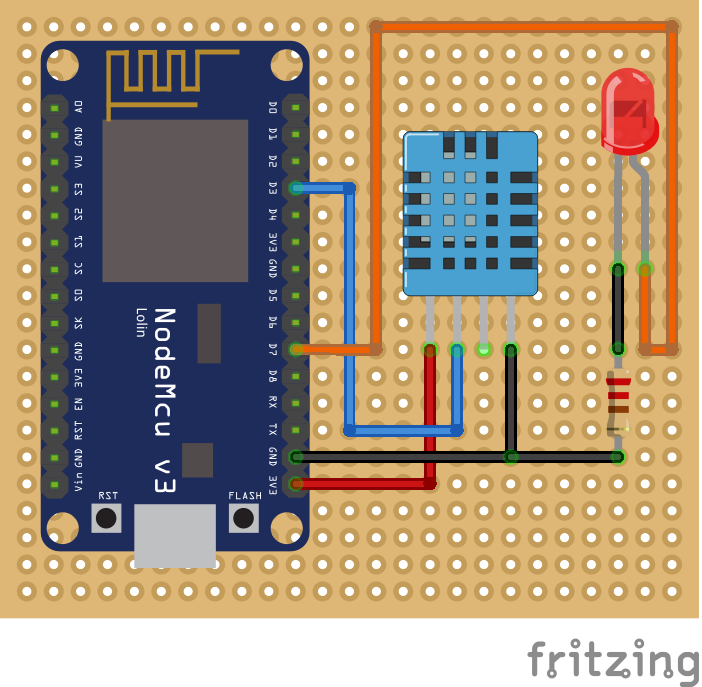
\includegraphics[width=0.6 \textwidth]{dht11.png}
  \caption{Schéma obvodu platformy NodeMCU, modulu DHT11 a led diody na plošném spoji}
  \label{fig:schema_esp_dht11}
\end{figure}

Fotografie fyzické realizace senzoru využívající modul DHT11 je na \cref{fig:nodemcu_ds18b20_dht11}. Modul DHT11 není úmyslně připájen přímo k plošnému spoji, ale je připojen přes konektor na desce. Během několika měsíců testovacího provozu přestalo fungovat jedno čidlo DHT11 a muselo být nahrazeno za jiné. Díky připojení přes dutinkovou lištu byla výměna modulu záležitostí několika vteřin. Tato výměna senzoru probíhá za provozu bez nutnosti restartu senzoru, senzor pomocí automatické detekce chyb pozná nefunkční čidlo a po výměně za nový kus sám naběhne do režimu čtení hodnot z modulu (více v \cref{sec:error_detection_esp}).

\subsection{Čidlo intenzity osvětlení TSL2591}

TSL2591 je čidlo sloužící pro měření intenzity osvětlení, které konvertuje intenzitu světla do digitálního výstupu přenášeného sběrnicí I$^2$C. Výstupem modulu je hodnota intenzity osvětlení v jednotce \si{lux} s přesností na 4 desetinná místa. Toto čidlo je jedno z nejdražších v projektu chytré domácnosti, ale nabízí víceméně dokonalé rozpoznání intenzity osvětlení od 188 $\mu$Lux do 88 000 Lux. Hodnota s přesností na 4 desetinná místa je zaokrouhlována na celá čísla, protože větší přesnost není vyžadována. Intenzita osvětlení v místnosti během dne se mění řádově o stovky luxů, v noci je osvětlení blízké 0 \si{lux}, přes den v rozmezí přibližně 30 až 500 \si{lux} a na přímém slunci je to několik desítek tisíc \si{lux}. Modul garantuje přesnost měření v teplotních podmínkách od -30 \si{\degree}C do +80 \si{\degree}C. Rozsah napájení desky s čidlem TSL2591 je od 3,3 V do 5,0 V. Velkou předností tohoto čidla je přítomnost diod pro měření infračerveného, celospektrálního a viditelného světla. \par
Každý modul TSL2591 má svou unikátní 7 bitovou adresu a komunikace s mikročipem ESP8266 probíhá přes I$^2$C sběrnici. K čidlu je přivedeno napájení z 3,3 V výstupu na mikročipu, dále je uzemněno GND drátem a I$^2$C komunikaci (výstupy SDA a SCL) s mikrokontrolérem zajišťují digitální GPIO piny D1 a D2. Schéma zapojení čidla TSL2591, platformy NodeMCU a externí led diody je zobrazeno na \cref{fig:schema_esp_tsl2591}.

\begin{figure}[H]
  \centering
  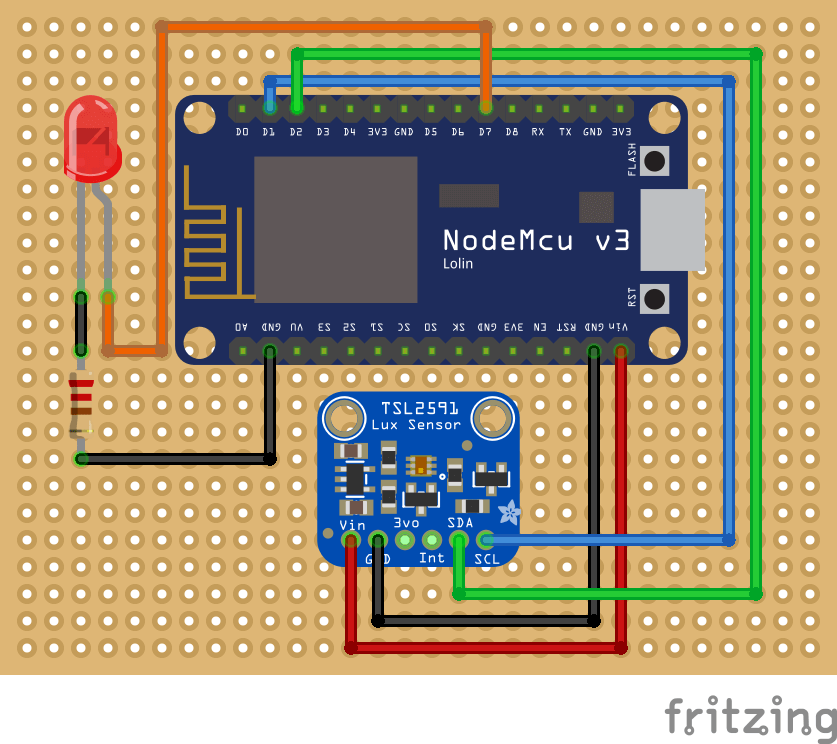
\includegraphics[width=0.6 \textwidth]{tsl2591.png}
  \caption{Schéma obvodu platformy NodeMCU, modulu TSL2591 a led diody na plošném spoji}
  \label{fig:schema_esp_tsl2591}
\end{figure}

Modul TSL2591 se během testování v projektu chytré domácnosti osvědčil pro svou kvalitu zpracování, přesnost naměřených hodnot, neobvykle velký rozsah měření a spolehlivost. Datová komunikace s tímto čidlem je výpočetně náročná, proto je použitý jeden samostatný mikročip ESP8266 pro obsluhu jen tohoto modulu. Fotografie zkonstruovaného senzoru je na \cref{fig:nodemcu_tsl2591}.

\begin{figure}[H]
  \centering
  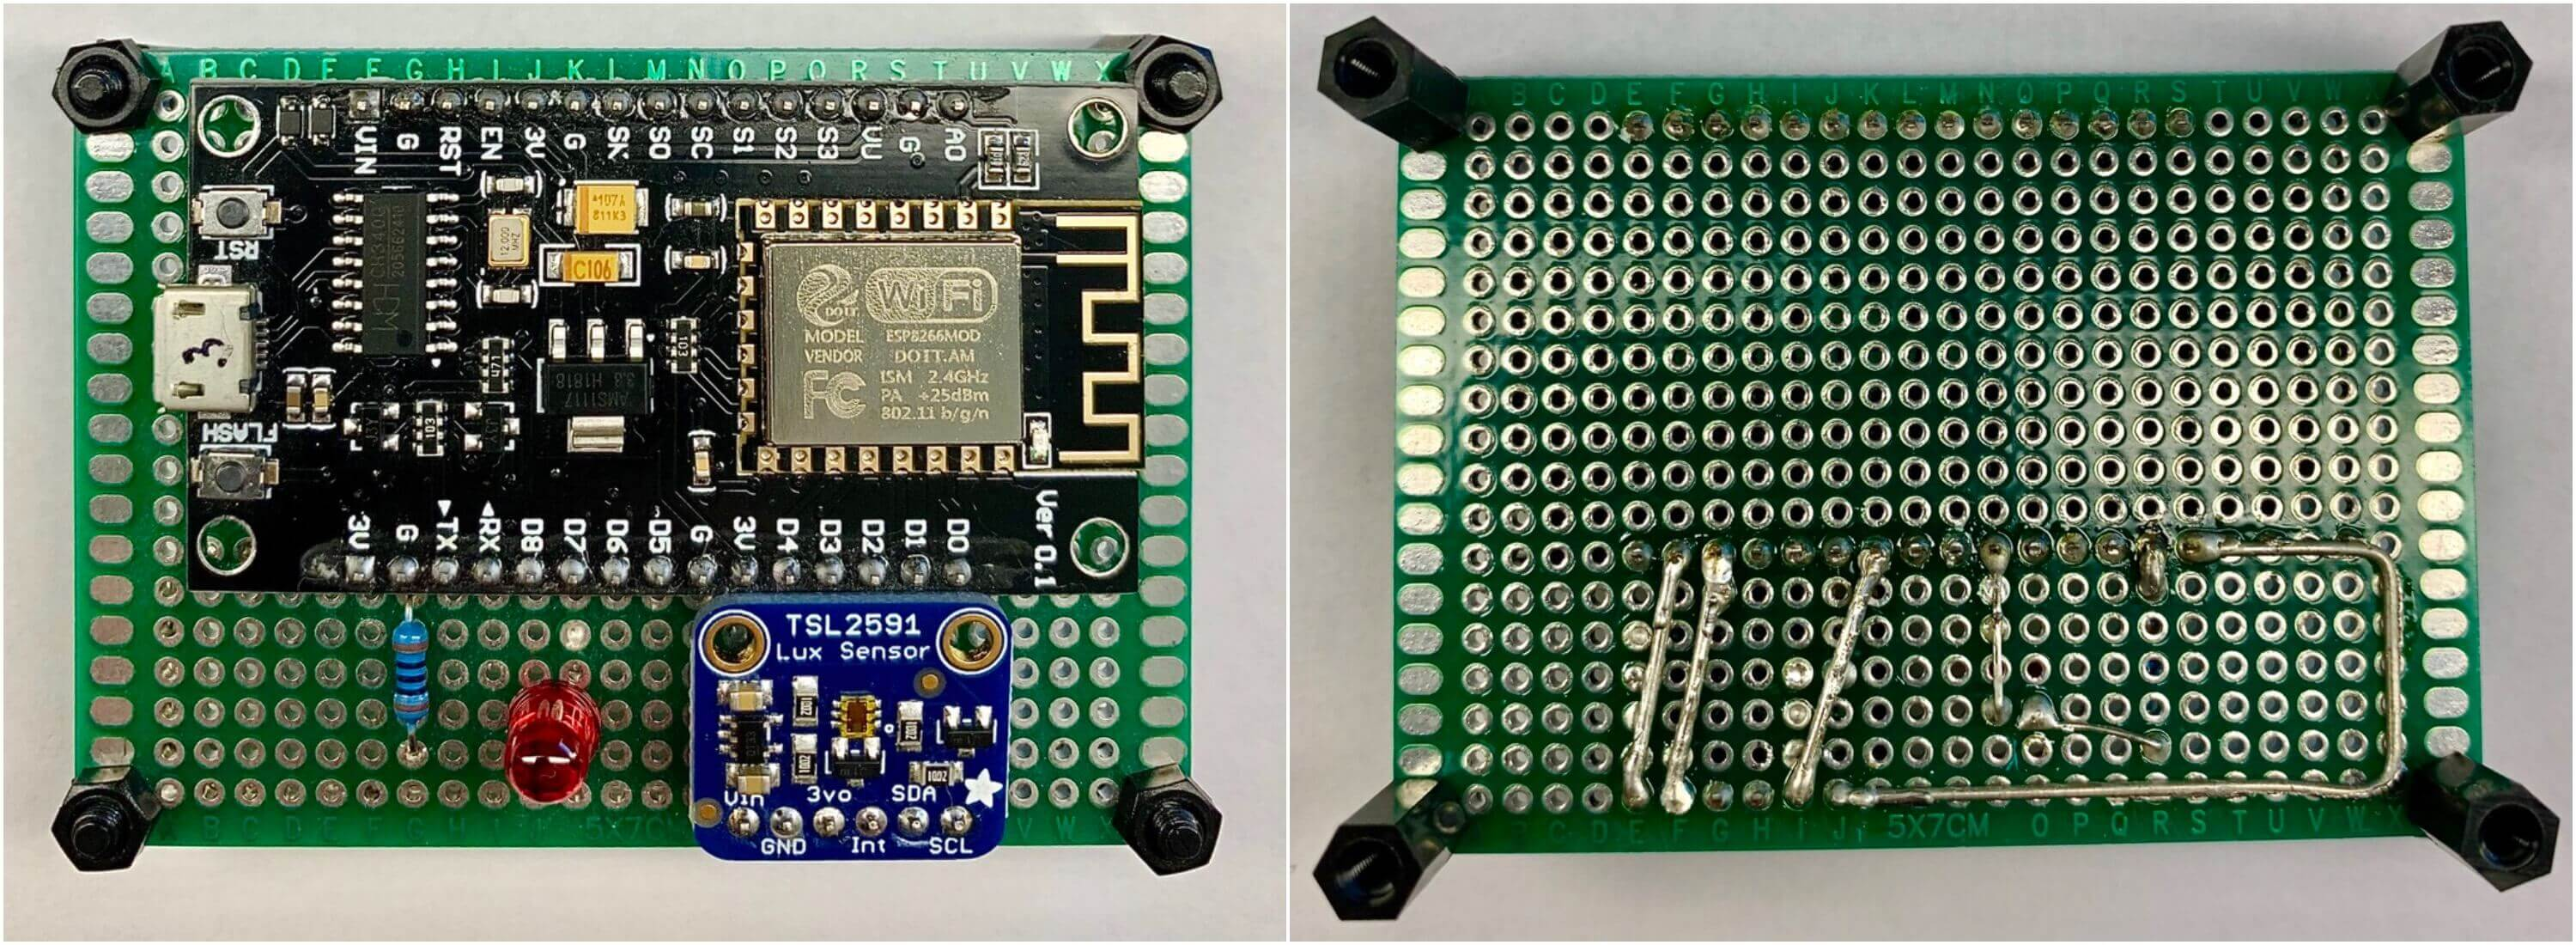
\includegraphics[width=0.85 \textwidth]{nodemcu_tsl2591.jpg}
  \caption{Fyzická realizace senzoru s modulem TSL2591}
  \label{fig:nodemcu_tsl2591}
\end{figure} 

\subsection{Čidlo barometrického tlaku a teploty BME280}

Modul BME280 od výrobce BOSH slouží k měření vnitřní teploty a barometrického tlaku. Čidlo je schopno měřit okolní teplotu v rozmezí -40 \si{\degree}C do +85 \si{\degree}C a barometrický tlak v rozsahu 300 \si{hPa} až 1100 \si{hPa}. Hodnoty teploty jsou měřeny s přesností $\pm$ 1 \si{\degree}C a hodnoty barometrického tlaku s přesností $\pm$ 1 \si{Pa}. Modul vrací zkonvertovanou hodnotu obou veličin s rozlišením na 2 desetinná místa. \par
Při porovnání naměřených hodnot teploty z čidla BME280 a z DS18B20 jsem zjistil, že hodnoty se liší v průměru o méně než 0,5 \si{\degree}C. Tento rozdíl je pro účely chytré domácnosti zanedbatelný a lze tedy předpokládat, že hodnoty teploty v místnosti jsou velmi přesné a čidlo DS18B20 pro běžné použití dostačuje, přestože je několikanásobně levnější, než modul BME280. Hodnoty barometrického tlaku je vhodné monitorovat s přesností na 2 desetinná místa, protože tato veličina se v místnosti v průběhu dne mění jen v minimálních mezích, za několik měsíců měření to průměrně bylo od 970 \si{hPa} do 980 \si{hPa}.\par
Komunikace s mikrokontrolérem probíhá po I$^2$C sběrnici. Reakční doba modulu od požadavku na změření hodnoty k odeslání hodnoty činí 1 vteřinu. S tímto zpožděním je opět nutno počítat při každém načítání hodnot. Kvůli výpočetní náročnosti při komunikaci s modulem a velikosti knihovny ovladače čidla je v tomto projektu využitý jeden samostatný mikročip ESP8266, který obsluhuje pouze toto čidlo. Schéma zapojení čidla BME280, platformy NodeMCU a externí led diody je zobrazeno na \cref{fig:schema_esp_bme280}.

\begin{figure}[H]
  \centering
  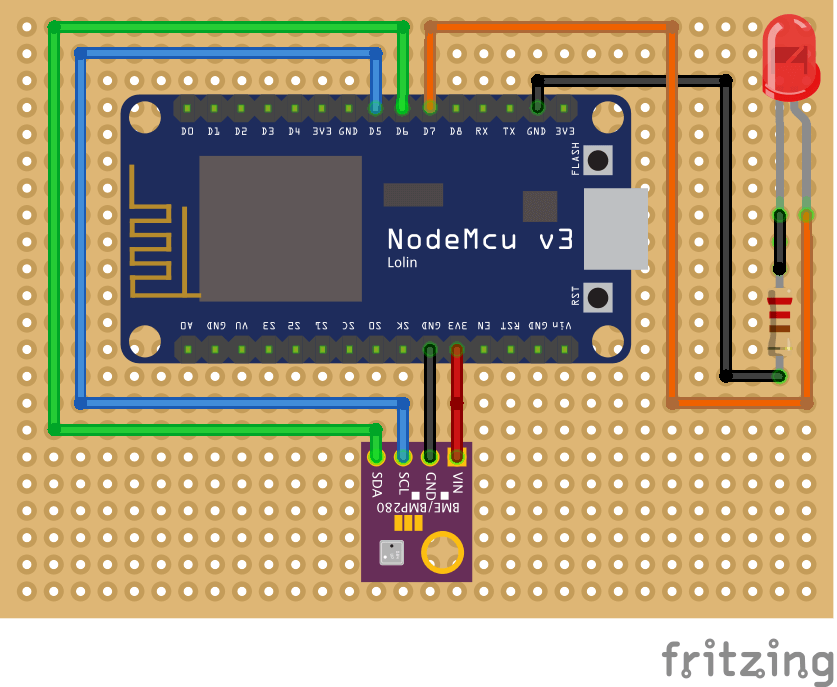
\includegraphics[width=0.5 \textwidth]{bme280.png}
  \caption{Schéma obvodu platformy NodeMCU, modulu BME280 a led diody na plošném spoji}
  \label{fig:schema_esp_bme280}
\end{figure}

Modul je k mikročipu ESP8266 připojen čtyřmi dráty - na výstup 3,3V pro napájení, GND pro uzemnění a dva digitální piny D5 a D6, které obstarávají přenos dat po sběrnici. Rozsah napájení desky s modulem BME280 je od 1,8 do 3,6 V. Senzor je umístěn na stole v rohu místnosti. Fotografie fyzické realizace senzoru je na \cref{fig:nodemcu_bme280}.

\begin{figure}[H]
  \centering
  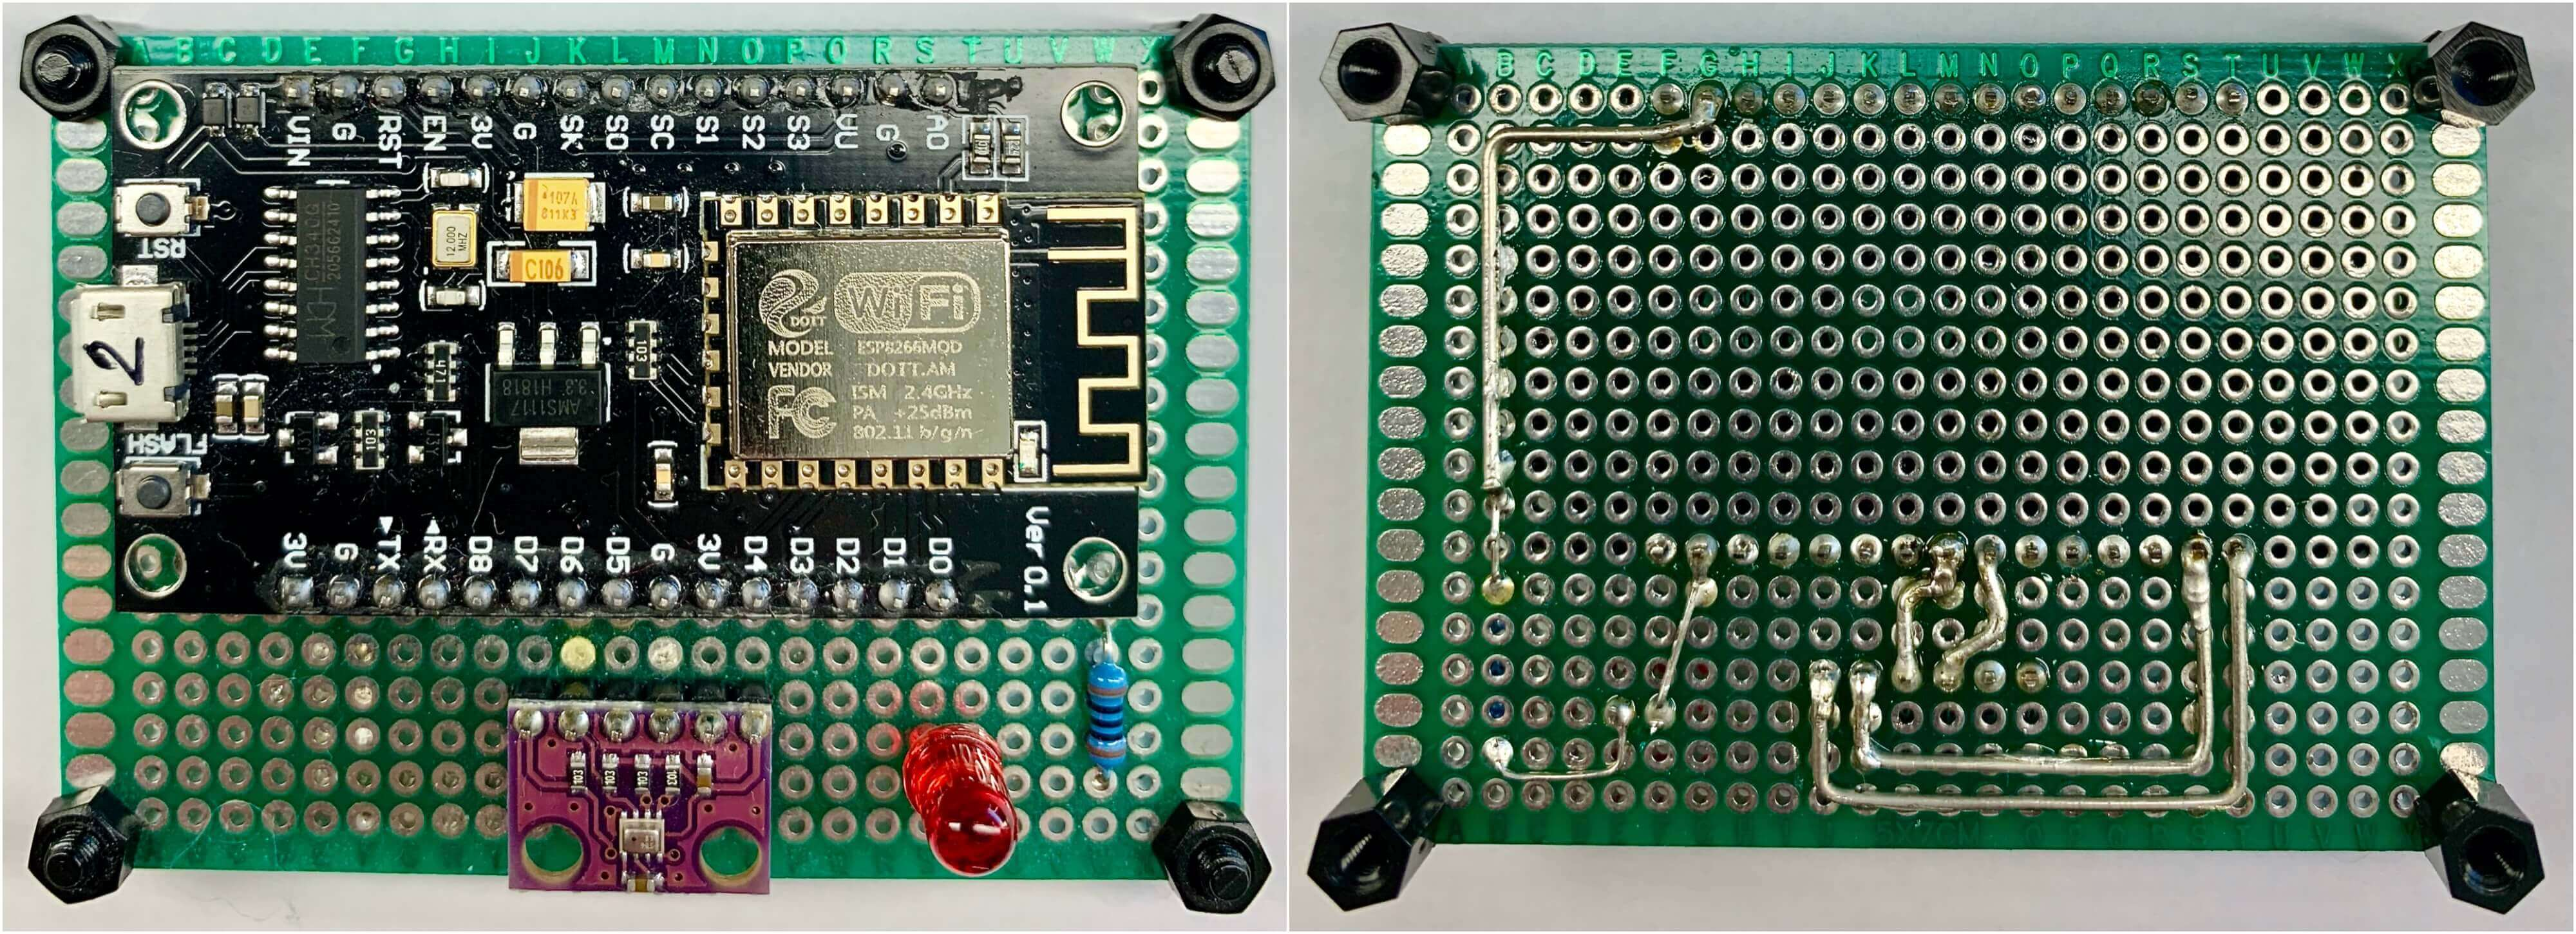
\includegraphics[width=0.9 \textwidth]{nodemcu_bme280.jpg}
  \caption{Fyzická realizace senzoru s modulem BME280}
  \label{fig:nodemcu_bme280}
\end{figure} 

\subsection{Pohybové čidlo AM312}

Modul pyroelektrické detekce pohybu AM312 slouží k monitorování pohybu osob v místnosti. Výstupem čidla je logická 1 v případě detekce pohybu a logická 0, pokud v místnosti není detekován pohyb. Jestliže v místnosti není detekován pohyb, čidlo neposílá žádnou informaci, výstupem na datovém pinu je trvale 0 a senzor čeká na vznik události (událost je v tomto případě detekce pohybu, více v \cref{subsec:event_based_msg}). Ve chvíli, kdy je detekován pohyb , dochází ke vzniku události a výstupem čidla je 1. Tento modul je rozměrově velmi kompaktní a pohyb detekuje ve vzdálenosti do 5 metrů. Úhel detekce pohybu je do 100 stupňů. V případě místností v chytré domácnosti je tato detekční vzdálenost a úhel dostačující. \par 
Modul AM312 se během několikaměsíčního provozu osvědčil pro svou spolehlivost. Pohyb byl detekován vždy, když jsem vstoupil do místnosti a zároveň modul neposílal falešné zprávy o pohybu v případě, že v domácnosti nikdo nebyl. Při experimentování s pohybovými čidly jsem testoval ještě modul HC-SR501, který má lepší specifikaci ve smyslu větší detekční vzdálenosti 7 m a úhlu do 120 stupňů, nicméně s tímto modulem byl problém právě s falešnými detekcemi. \par
Čidlo AM312 je konstruováno pro vstupní napětí od 2,7 do 12 V a pro prostřední s okolní teplotou od -20 \si{\degree}C do +60 \si{\degree}C. K mikrokontroléru ESP8266 je připojeno třemi dráty - jeden k vývodu 3,3 V pro napájení, jeden k GND výstupu pro uzemnění a jeden k digitálnímu pinu D8 pro přenos informace. Na plošném spoji tohoto senzoru je navíc přidán externí bzučák, který má využití jako alarm v případě detekce pohybu. Tento zvukový signál se hodil spíše pro prvotní ladění a testování na falešné poplachy, po odladění se jako vizuální signalizace detekce pohybu využívala externí led dioda, která se při zaznamenání pohybu rozsvítí na dobu 2 vteřin. Touto indikací jsem si ověřoval správnou funkčnost senzoru. Schéma zapojení pohybového čidla AM312, platformy NodeMCU, externí led diody a externího bzučáku na plošném spoji je na \cref{fig:schema_esp_am312}. 

\begin{figure}[H]
  \centering
  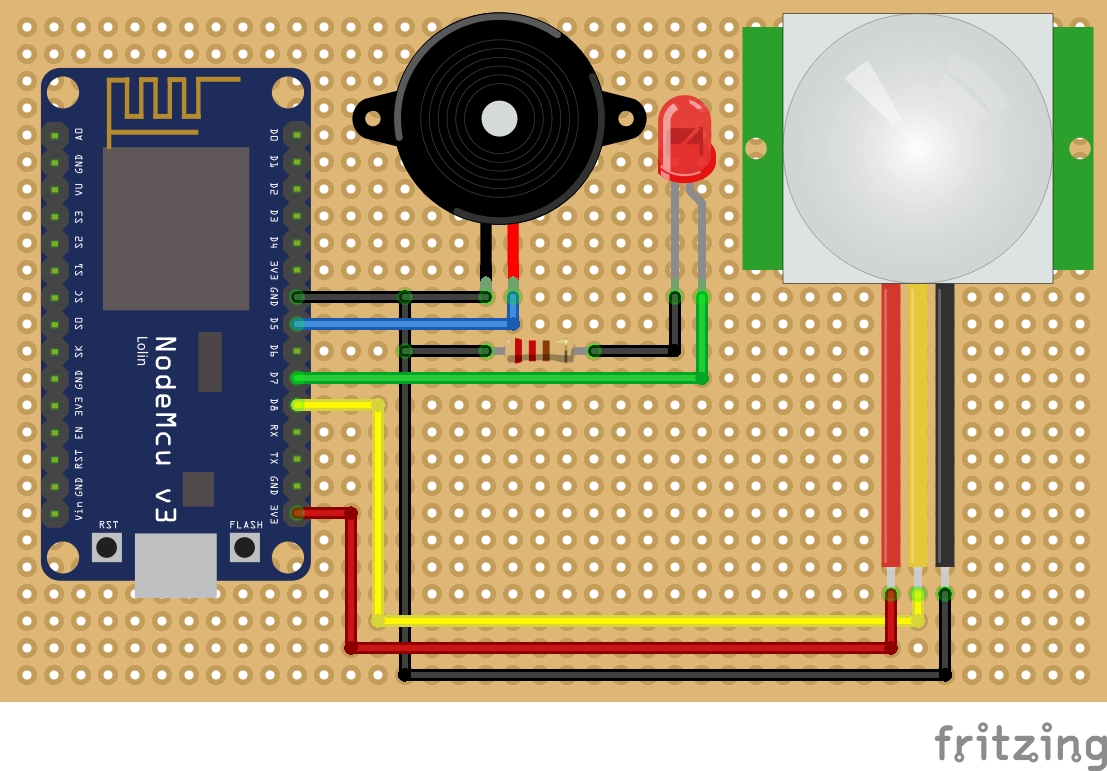
\includegraphics[width=0.6 \textwidth]{am312.png}
  \caption{Schéma obvodu platformy NodeMCU, modulu AM312, led diody a externího bzučáku na plošném spoji}
  \label{fig:schema_esp_am312}
\end{figure}

Za účelem efektivní detekce je senzor umístěn v rohu místnosti naproti dveřím. Toto specifické umístění nedovoluje využití mikročipu ESP8266 současně s jiným senzorem, ale v tomto případě by to ani nebylo žádané. Pohybový senzor je jedním ze dvou senzorů, které odesílají zprávy na základě vzniku události (více v \cref{subsec:event_based_msg}). Tento přístup nelze efektivně kombinovat s periodickým odesíláním další veličiny. Fotografie fyzické realizace senzoru je na \cref{fig:nodemcu_am312}.

\begin{figure}[H]
  \centering
  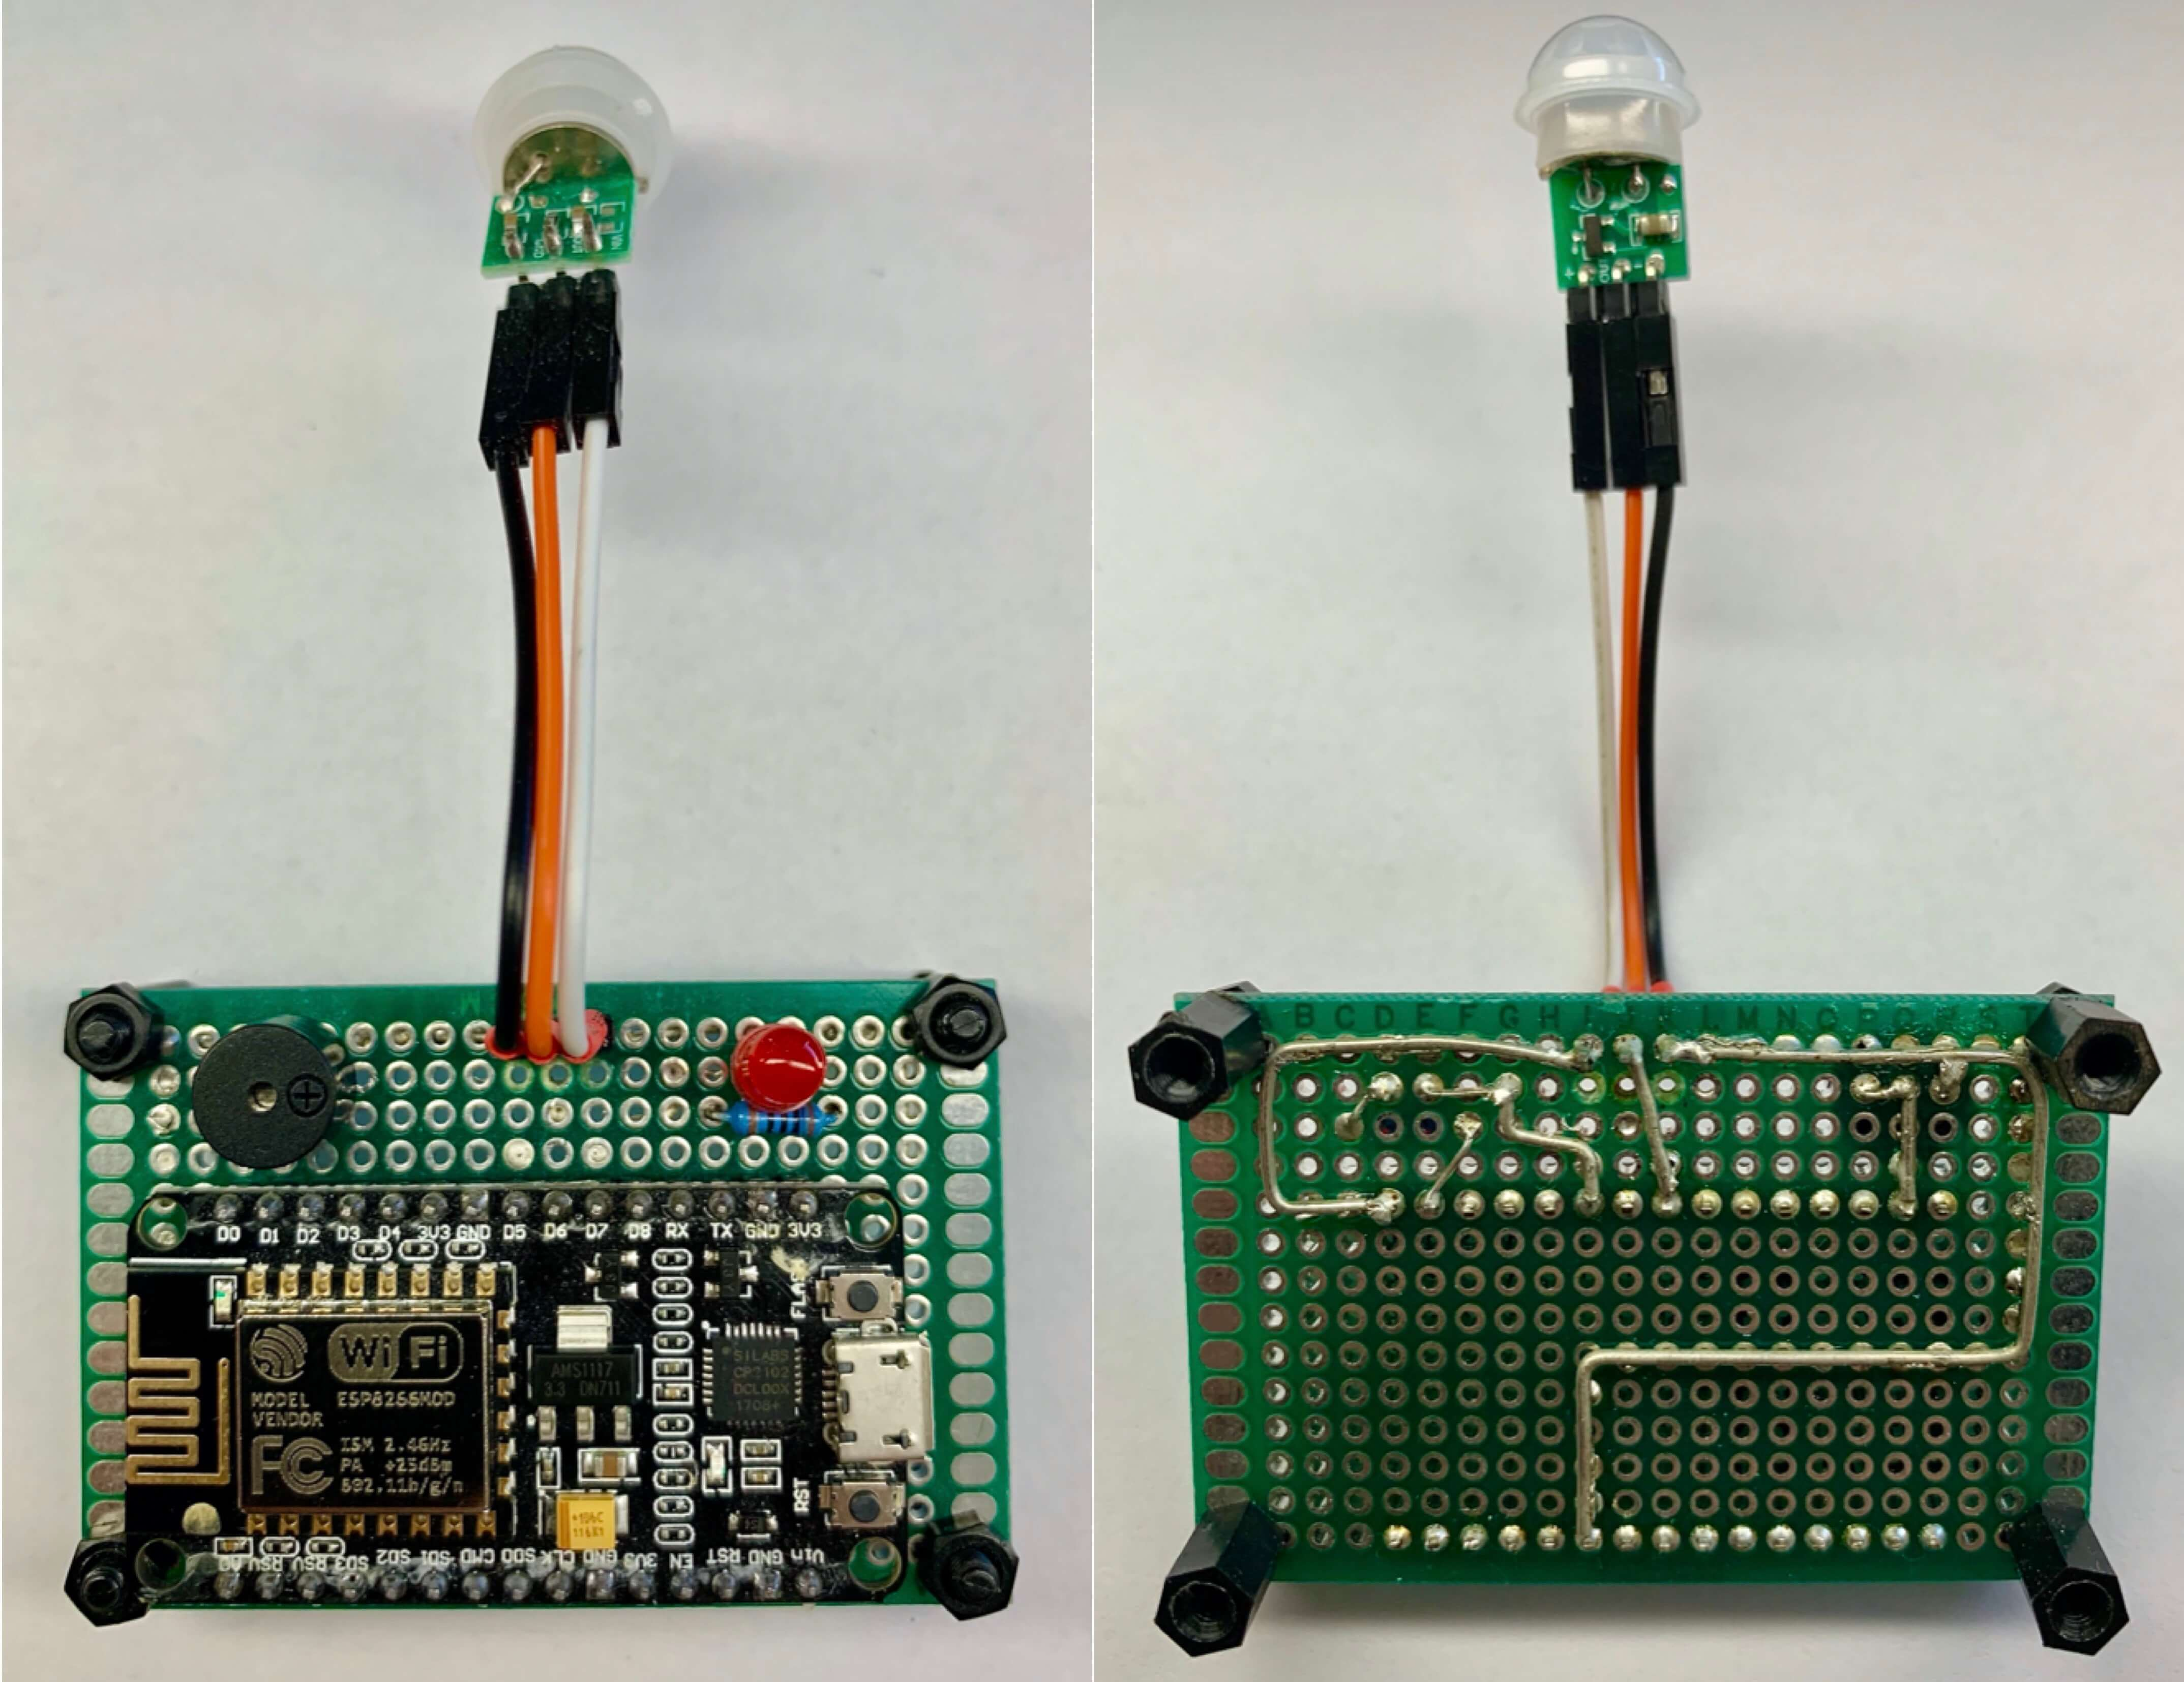
\includegraphics[width=0.7 \textwidth]{nodemcu_am312.jpeg}
  \caption{Fyzická realizace senzoru s modulem AM312}
  \label{fig:nodemcu_am312}
\end{figure} 

\subsection{Magnetické čidlo LS311B38}
Magnetický jazýčkový kontakt LS311B38 slouží k detekci otevřeného okna nebo otevřených dveří. Toto čidlo je jedním z nejjednodušších čidel v projektu chytré domácnosti. Jedná se o 2 kusy magnetu, jedna část je umístěna na okně nebo dveřích a druhá část je připevněna k okennímu nebo nebo \mbox{dveřnímu} rámu. Magnety musejí být umístěny tak, že když je okno zavřené, oba kusy magnetu jsou blízko u sebe. Výstupem tohoto čidla je logická 1 v případě, že jsou magnety blízko u sebe (zavřené okno nebo zavřené dveře) nebo logická 0 v případě, kdy jsou magnetické jazýčky rozpojeny. V projektu chytré domácnosti je monitorován stav jednoho okna a jedněch dveří. Pro tuto realizaci je využitý jeden mikrokontrolér ESP8266, který obsluhuje oba magnetické kontakty. Na plošném spoji jsou dvě externí led diody, jedna slouží pro vizuální indikaci otevřených dveří, druhá pro indikaci otevřeného okna. \par
Spínací vzdálenost magnetů je od 15 mm do 25 mm. Princip zapojení magnetických jazýčku k mikročipu ESP8266 je velmi podobný zapojení tlačítka. Z magnetu vedou dva kabely, které jsou připájeny k výstupům GND pro uzemnění a digitálnímu pinu D7. Oba kabely vedou jen z jednoho kusu magnetu a mikročip čeká na přiblížení druhého magnetu, čímž se obvod spojí a signál je přes digitální pin přenesen do mikročipu. Schéma zapojení magnetického kontaktu LS311B38, platformy NodeMCU a externí led diody je zobrazen na \cref{fig:schema_esp_ls311b38}.

\begin{figure}[H]
  \centering
  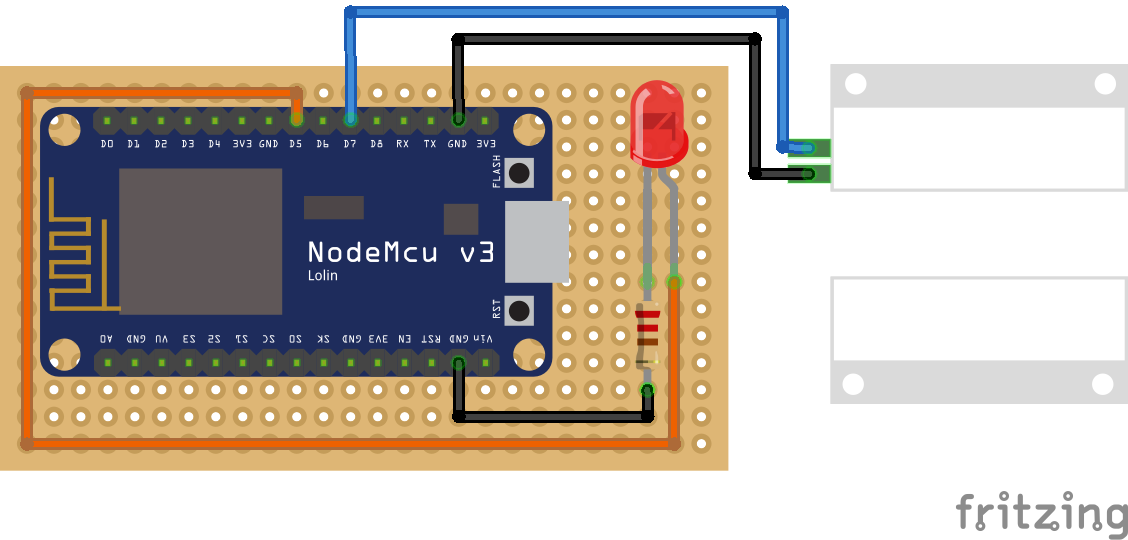
\includegraphics[width=0.6 \textwidth]{ls311b38.png}
  \caption{Schéma obvodu platformy NodeMCU, magnetického kontaktu LS311B38 a led diody na plošném spoji}
  \label{fig:schema_esp_ls311b38}
\end{figure}

Vzhledem k jednoduchosti čidla lze předpokládat velmi dlouhou životnost a spolehlivost. Fotografie fyzické realizace senzoru je na \cref{fig:nodemcu_ls311b38}.

\begin{figure}[H]
  \centering
  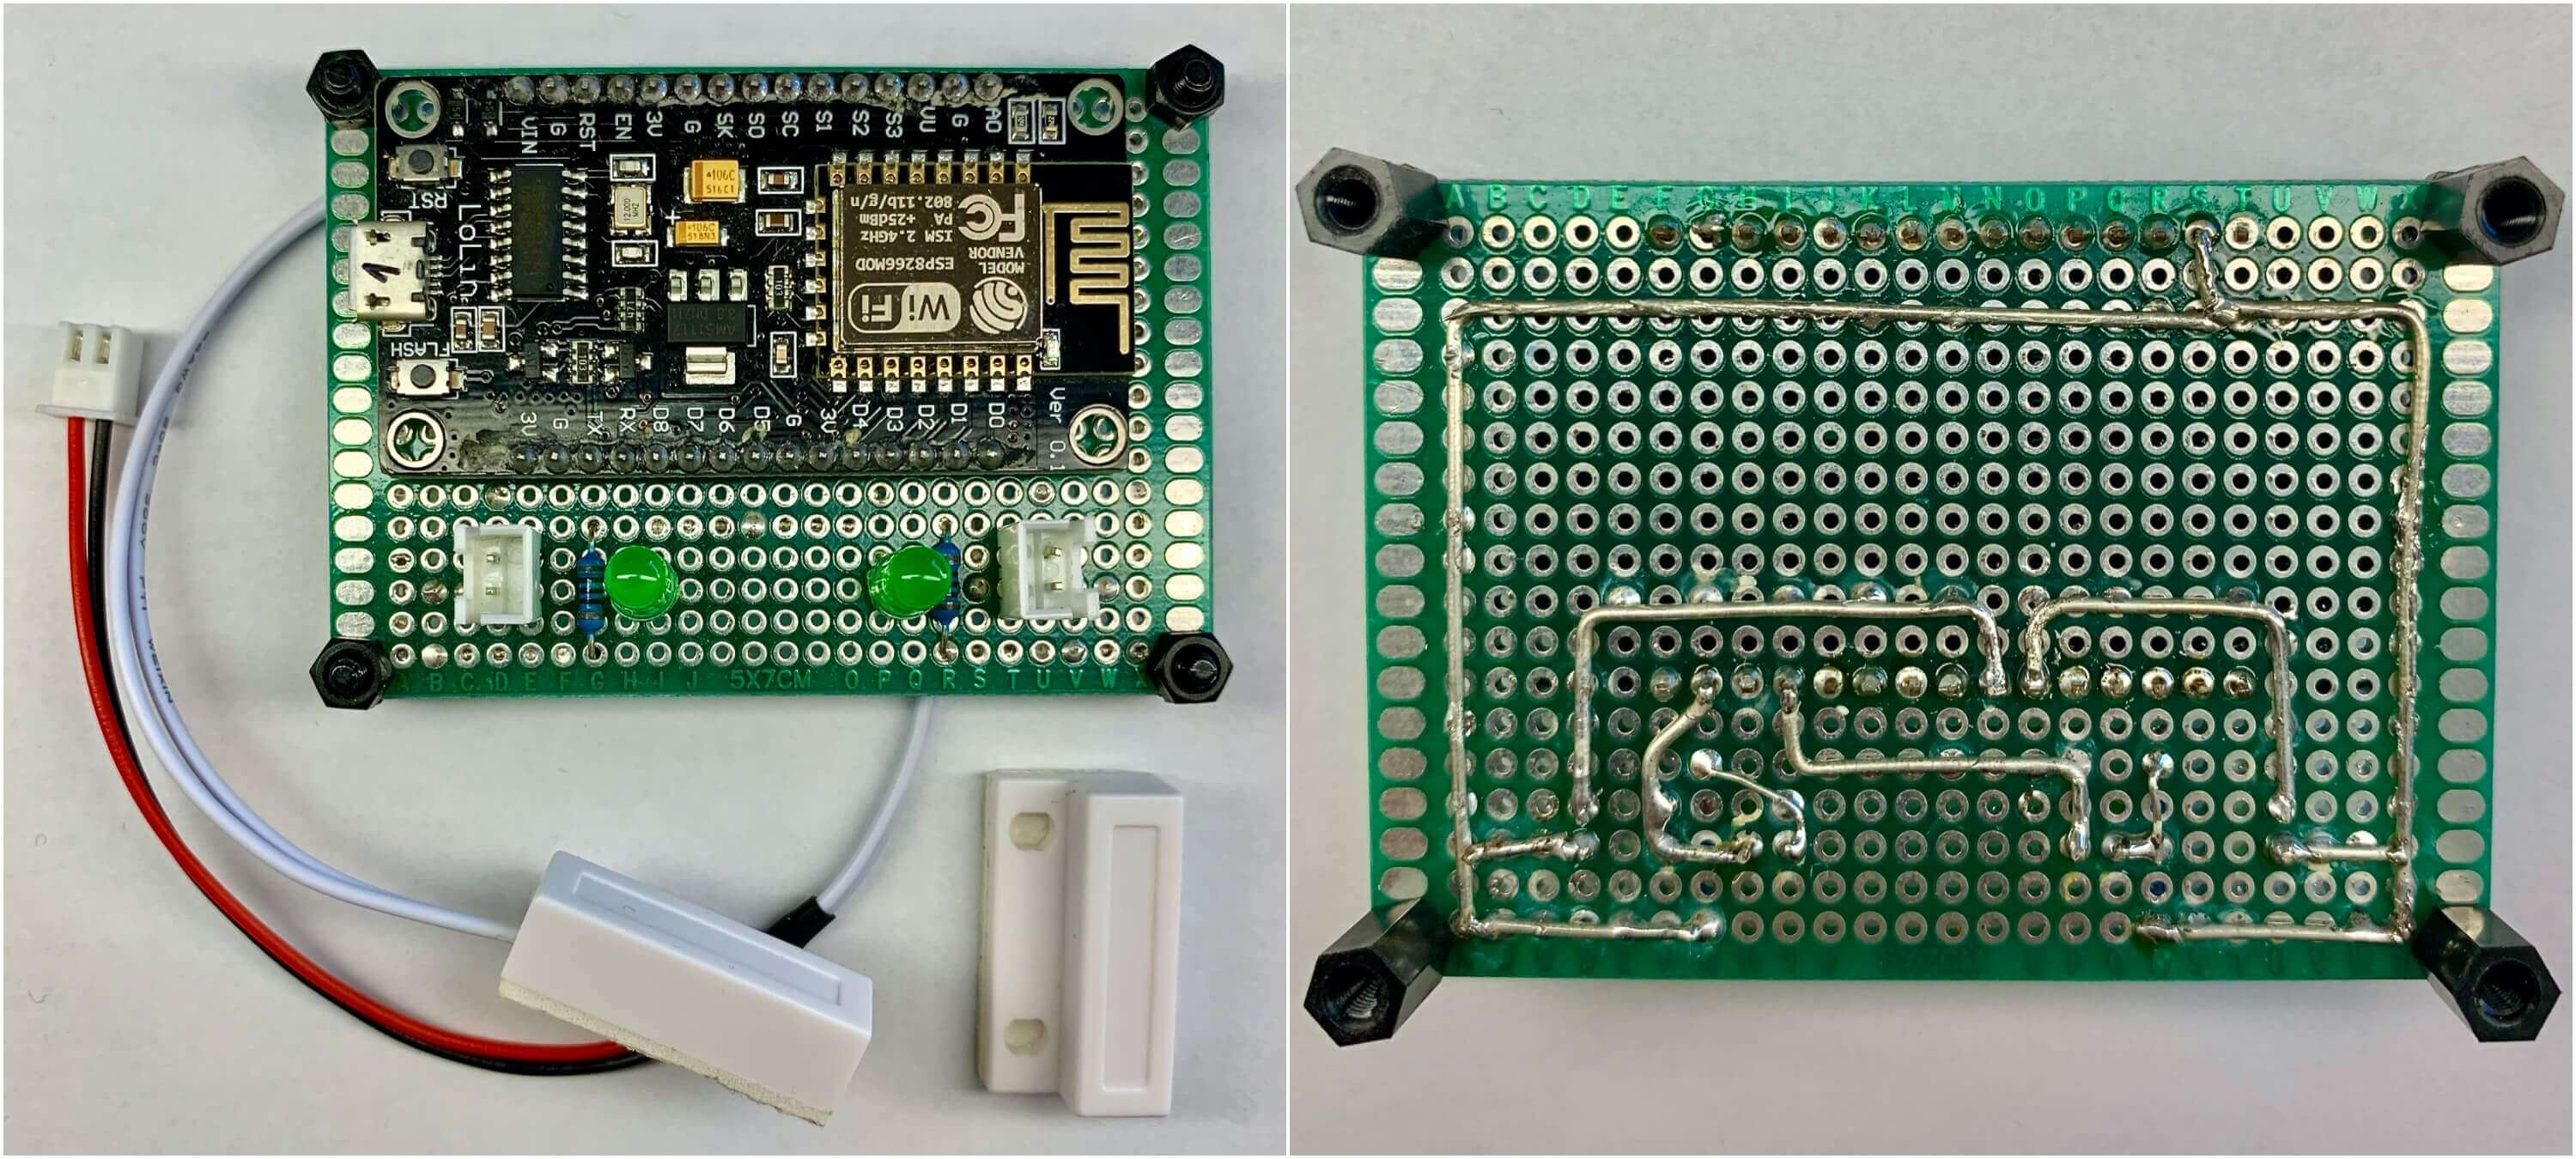
\includegraphics[width=0.8 \textwidth]{nodemcu_ls311b38.jpg}
  \caption{Fyzická realizace senzoru s magnetickým kontaktem LS311B38}
  \label{fig:nodemcu_ls311b38}
\end{figure} 

\section{Raspberry Pi} \label{sec:raspberry_pi}
\textit{Raspberry Pi} je jednočipový počítač s operačním systémem Raspbian. Raspbian OS je založený na Linuxu a po instalaci nabízí podporu několika programovacích jazyků a je přímo přizpůsoben na DIY projekty. Základní deska umožňuje připojit externí monitor pomocí microHDMI a externí komponenty jako je klávesnice a myš přes USB. K místní síti se připojuje klasickým LAN kabelem s koncovkou RJ45 nebo bezdrátově přes Wi-Fi. Oproti mikrokontrolérům jako jsou čipy ESP8266 nebo Arduino nabízí kromě ovládání příslušenství pomocí GPIO kontaktů hlavně možnost programovat samotné aplikace. V projektu chytré domácnosti byla použita v současné době nejvýkonnější verze počítače Raspbery Pi 4 - Model B s 4 GB RAM, který byl uveden do prodeje v červnu 2019. Tento model je osazen 1,5 GHz čtyřjádrovým procesorem ARM Cortex-A72 a jako externí monitor lze použít displej s rozlišením 4K při 60 snímcích za vteřinu. Operační systém je nainstalován na externí microSD kartě s kapacitou 32 GB. Tato nejvýkonnější konfigurace byla zvolena z důvodu vytíženosti RPi v projektu chytré domácnosti. 

\begin{figure}[H]
  \centering
  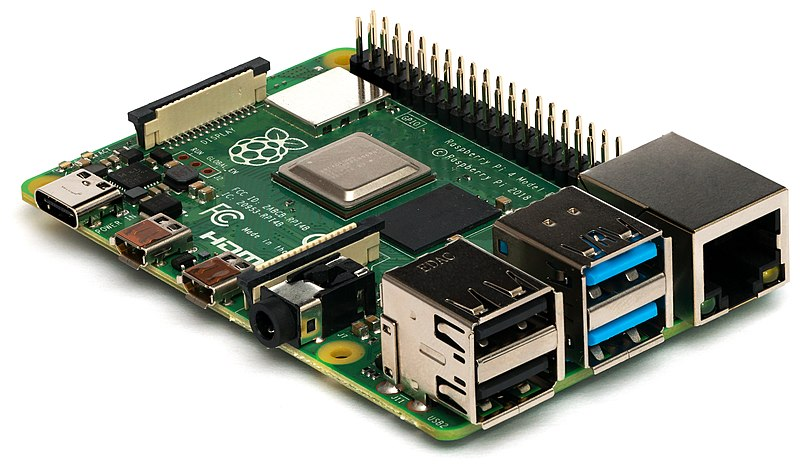
\includegraphics[width=0.5 \textwidth]{raspberry_pi.jpg}
  \caption{Jednočipový počítač Raspberry Pi 4 Model B}
  \label{fig:raspberry_pi}
\end{figure} 

\subsection*{Využití v chytré domácnosti}
Počítač Raspberry Pi má v projektu chytré domácnosti několik využití. 

\begin{itemize}
  \item MQTT Broker
  \item Databázový server
  \item Trénování modelů a klasifikace
  \item Web server
\end{itemize}

Primárně slouží jako MQTT broker, který přijímá všechny příchozí zprávy ze senzorů (více v \cref{sec:protocol_mqtt}). Dále na RPi běží databázový server za účelem ukládání všech příchozích zpráv do databáze (více v \cref{sec:database}). Současně jsou na RPi trénovány modely, na základě kterých je prováděna klasifikace jednotlivých příchozích zpráv (více v \cref{sec:detection_classification}). Datově náročnější modely lze trénovat na externích výkonnějších počítačích a následně na RPi použít pro klasifikaci již natrénované modely. Za účelem grafické vizualizace naměřených dat a aktuálních hodnot veličin běží na RPi webový server (více v \cref{sec:webserver}). 

Velkou výhodou RPi jsou minimální rozměry a hlavně malý odběr proudu. V těchto aplikacích je nutné, aby počítač byl neustále zapnutý. Klasické PC by se k těmto účelům nehodilo kvůli vysoké spotřebě a nepotřebně velkému výkonu. Náklady na provoz a pořízení počítače RPi jsou ve srovnání s klasickém PC serverem několikanásobně nižší. 

Raspberry Pi 4 Model B má i v tomto případě, kdy na RPi probíhá několik procesů paralelně vedle sebe, dostatečný výkon. Doba počítání modelů a klasifikace zpráv je v rámci vteřin, narozdíl od starších modelů RPi. Nevýhodou tohoto přístupu, kdy jeden server slouží k několika účelům, je nebezpečí pádu celého systému, pokud server přestane pracovat. V případě, že z nějakého důvodu přestane pracovat RPi, přestanou se do databáze ukládat všechny příchozí zprávy, nově příchozí zprávy tudíž nebudou ani klasifikovány a webová vizualizace bude nedostupná. V případě nedostupnosti webové vizualizace pravděpodobně nejde o velký problém, ale pokud nejsou příchozí zprávy ukládány do databáze delší dobu, jde o závažnější problém a výsledné modely mohou být zkresleny. Tuto nevýhodu je vhodné vyřešit rozdělením procesů na více strojů - na více RPi. V této práci byla všechna data zálohována do cloudu.